% Soubory musí být v kódování, které je nastaveno v příkazu \usepackage[...]{inputenc}

\documentclass[%        Základní nastavení
%  draft,    				  % Testovací překlad
  12pt,       				% Velikost základního písma je 12 bodů
  a4paper,    				% Formát papíru je A4
  oneside,      			% Jednostranný tisk
	% twoside,      			% Dvoustranný tisk (kapitoly a další důležité části tedy začínají na lichých stranách)
	unicode,						% Záložky a metainformace ve výsledném  PDF budou v kódování unicode
]{report}				    	% Dokument třídy 'zpráva', vhodná pro sazbu závěrečných prací s kapitolami

\usepackage[utf8]		  %	Kódování zdrojových souborů je UTF-8
	{inputenc}					% Balíček pro nastavení kódování zdrojových souborů

\usepackage[				% Nastavení geometrie stránky
	bindingoffset=10mm,		% Hřbet pro vazbu
	hmargin={25mm,25mm},	% Vnitřní a vnější okraj  (jsou nehezky shodné; jakási úroveň estetiky je dosažena pomocí hřbetu)
	vmargin={25mm,34mm},	% Horní a dolní okraj
	footskip=17mm,			  % Velikost zápatí
	nohead,					      % Bez záhlaví
	marginparsep=2mm,		  % Vzdálenost marginálií
	marginparwidth=18mm,	% Šířka marginálií
]{geometry}

\usepackage{sectsty}
	%přetypuje nadpisy všech úrovní na bezpatkové, kromě \chapter, která je přenastavena zvlášť v thesis.sty
	\allsectionsfont{\sffamily}

\usepackage{graphicx} % Balíček 'graphicx' pro vkládání obrázků
											% Nutné pro vložení logotypů školy a fakulty

\usepackage[          % Balíček 'acronym' pro sazby zkratek a symbolů
	nohyperlinks				% Nebudou tvořeny hypertextové odkazy do seznamu zkratek
]{acronym}						
											% Nutné pro použití prostředí 'acronym' balíčku 'thesis'

\usepackage[
	breaklinks=true,		% Hypertextové odkazy mohou obsahovat zalomení řádku
	hypertexnames=false, % Názvy hypertext. odkazů budou tvořeny nezávisle na názvech TeXu
]{hyperref}						% Balíček 'hyperref' pro sazbu hypertextových odkazů
											% Nutné pro použití příkazu 'pdfsettings' balíčku 'thesis'

\usepackage{pdfpages} % Balíček umožňující vkládat stránky z PDF souborů
                      % Nutné při vkládání titulních listů a zadání přímo
                      % ve formátu PDF z informačního systému

\usepackage{enumitem} % Balíček pro nastavení mezerování v odrážkách
  \setlist{topsep=0pt,partopsep=0pt,noitemsep} % konkrétní nastavení

\usepackage{cmap} 		% Balíček cmap zajišťuje, že PDF vytvořené `pdflatexem' je
											% plně "prohledávatelné" a "kopírovatelné"

%\usepackage{upgreek}	% Balíček pro sazbu stojatých řeckých písmem
											%% např. stojaté pí: \uppi
											%% např. stojaté mí: \upmu (použitelné třeba v mikrometrech)
											%% pozor, grafická nekompatibilita s fonty typu Computer Modern!
                      
%\usepackage{amsmath} %balíček pro sabu náročnější matematiky                 

\usepackage{dirtree}	% sazba adresářové struktury
                      % vhodné pro prezentaci obsahu elektronické přílohy (např. CD)

\usepackage[formats]{listings}	% Balíček pro sazbu zdrojových textů
\lstset{              % nastavení
%	Definice jazyka použitého ve výpisech
%    language=[LaTeX]{TeX},	% LaTeX
%	language={Matlab},		% Matlab
	language={C},           % jazyk C
    basicstyle=\ttfamily,	% definice základního stylu písma
    tabsize=2,			% definice velikosti tabulátoru
    inputencoding=utf8,         % pro soubory uložené v kódování UTF-8
		columns=fixed,  %fixed nebo flexible,
		fontadjust=true %licovani sloupcu
    extendedchars=true,
    literate=%  definice symbolů s diakritikou
    {á}{{\'a}}1
    {č}{{\v{c}}}1
    {ď}{{\v{d}}}1
    {é}{{\'e}}1
    {ě}{{\v{e}}}1
    {í}{{\'i}}1
    {ň}{{\v{n}}}1
    {ó}{{\'o}}1
    {ř}{{\v{r}}}1
    {š}{{\v{s}}}1
    {ť}{{\v{t}}}1
    {ú}{{\'u}}1
    {ů}{{\r{u}}}1
    {ý}{{\'y}}1
    {ž}{{\v{z}}}1
    {Á}{{\'A}}1
    {Č}{{\v{C}}}1
    {Ď}{{\v{D}}}1
    {É}{{\'E}}1
    {Ě}{{\v{E}}}1
    {Í}{{\'I}}1
    {Ň}{{\v{N}}}1
    {Ó}{{\'O}}1
    {Ř}{{\v{R}}}1
    {Š}{{\v{S}}}1
    {Ť}{{\v{T}}}1
    {Ú}{{\'U}}1
    {Ů}{{\r{U}}}1
    {Ý}{{\'Y}}1
    {Ž}{{\v{Z}}}1
}

%%%%%%%%%%%%%%%%%%%%%%%%%%%%%%%%%%%%%%%%%%%%%%%%%%%%%%%%%%%%%%%%%
%%%%%%      !!! VLASTNÍ BALÍČKY A NASTAVENÍ !!!        %%%%%%%%%%
%%%%%%%%%%%%%%%%%%%%%%%%%%%%%%%%%%%%%%%%%%%%%%%%%%%%%%%%%%%%%%%%%
%====== Units =====
\usepackage{siunitx}
\sisetup{inter-unit-product =\ensuremath{\cdot}}
\sisetup{group-digits = integer}
\sisetup{output-decimal-marker = {,}}
\sisetup{exponent-product = \ensuremath{\cdot}}
\sisetup{separate-uncertainty}
\sisetup{tight-spacing = false}
\DeclareSIUnit\permille{\text{\textperthousand}}
%\sisetup{scientific-notation = true}
%\sisetup{round-mode=places,round-precision=4}
%\sisetup{evaluate-expression}

%====== Hyperlinky ====== 
\hypersetup{allbordercolors={1 1 1}}

%====== Obrazky ========
% \usepackage{graphicx} 
% \usepackage[dvipsnames]{xcolor} % E: option clash for package xcolor
% \usepackage{tikz}

% ^^ už tam někde prý jsou použité

\usepackage[siunitx]{circuitikz}
\usepackage{pgf}
\usetikzlibrary{matrix}
\usetikzlibrary{fit}
\usetikzlibrary{patterns}
\usepackage{tkz-euclide}
\usetikzlibrary{arrows.meta, bending, patterns.meta, ducks}
\usetikzlibrary{shapes, backgrounds, decorations.pathmorphing, calc}
\usetikzlibrary{positioning}

\usepackage{derivative} % nebude potřeba

\usepackage{pgfplots}
\pgfplotsset{width=0.8\linewidth, compat=1.17}
\def\plotcscale{0.8}
\usepackage{pgfplotstable}
\newcommand*\circled[1]{\tikz[baseline=(char.base)]{
            \node[shape=circle,draw,inner sep=1pt] (char) {#1};}}

\usepackage[style=iso-numeric,backend=biber]{biblatex}
\addbibresource{text/literatura.bib}
%making everything to match Juice citations
\DeclareFieldFormat{labelnumberwidth}{\mkbibbrackets{#1}}
% \usepackage{natbib}
% \usepackage{url}
% \DeclareUrlCommand\url{\def\UrlLeft{<}\def\UrlRight{>} \urlstyle{tt}}


% TEMP
\usepackage{multirow}
\usepackage{array}
\usepackage{tabularx}
\usepackage{calc}





%%%%%%%%%%%%%%%%%%%%%%%%%%%%%%%%%%%%%%%%%%%%%%%%%%%%%%%%%%%%%%%%%
%%%%%%      Definice informací o dokumentu             %%%%%%%%%%
%%%%%%%%%%%%%%%%%%%%%%%%%%%%%%%%%%%%%%%%%%%%%%%%%%%%%%%%%%%%%%%%%

% V tomto souboru se nastavují téměř veškeré informace, proměnné mezi studenty:
% jméno, název práce, pohlaví atd.
% Tento soubor je SDÍLENÝ mezi textem práce a prezentací k obhajobě -- netřeba něco nastavovat na dvou místech.

\usepackage[
%%% Z následujících voleb jazyka lze použít pouze jednu
  czech-english,		% originální jazyk je čeština, překlad je anglicky (výchozí)
  %english-czech,	% originální jazyk je angličtina, překlad je česky
  %slovak-english,	% originální jazyk je slovenština, překlad je anglicky
  %english-slovak,	% originální jazyk je angličtina, překlad je slovensky
%
%%% Z následujících voleb typu práce lze použít pouze jednu
  % semestral,		  % semestrální práce (výchozí)
  bachelor,			%	bakalářská práce
  %master,			  % diplomová práce
  %treatise,			% pojednání o disertační práci
  %doctoral,			% disertační práce
%
%%% Z následujících voleb zarovnání objektů lze použít pouze jednu
%  left,				  % rovnice a popisky plovoucích objektů budou zarovnány vlevo
	center,			    % rovnice a popisky plovoucích objektů budou zarovnány na střed (vychozi)
%
]{thesis}   % Balíček pro sazbu studentských prací


%%% Jméno a příjmení autora ve tvaru
%  [tituly před jménem]{Křestní}{Příjmení}[tituly za jménem]
% Pokud osoba nemá titul před/za jménem, smažte celý řetězec '[...]'
\author{Jakub}{Charvot}

%%% Identifikační číslo autora (VUT ID)
\butid{240844}

%%% Pohlaví autora/autorky
% (nepoužije se ve variantě english-czech ani english-slovak)
% Číselná hodnota: 1...žena, 0...muž
\gender{0}

%%% Jméno a příjmení vedoucího/školitele včetně titulů
%  [tituly před jménem]{Křestní}{Příjmení}[tituly za jménem]
% Pokud osoba nemá titul před/za jménem, smažte celý řetězec '[...]'
\advisor[Ing.]{Pavel}{Tomíček}

%%% Jméno a příjmení oponenta včetně titulů
%  [tituly před jménem]{Křestní}{Příjmení}[tituly za jménem]
% Pokud osoba nemá titul před/za jménem, smažte celý řetězec '[...]'
% Nastavení oponenta se uplatní pouze v prezentaci k obhajobě;
% v případě, že nechcete, aby se na titulním snímku prezentace zobrazoval oponent, pouze příkaz zakomentujte;
% u obhajoby semestrální práce se oponent nezobrazuje (jelikož neexistuje)
% U dizertační práce jsou typicky dva až tři oponenti. Pokud je chcete mít na titulním slajdu, prosím ručně odkomentujte a upravte jejich jména v definici "VUT title page" v souboru thesis.sty.
% TODO:
\opponent[Ing.]{Vladimír}{Levek}[Ph.D.]

%%% Název práce
%  Parametr ve složených závorkách {} je název v originálním jazyce,
%  parametr v hranatých závorkách [] je překlad (podle toho jaký je originální jazyk).
%  V případě, že název Vaší práce je dlouhý a nevleze se celý do zápatí prezentace, použijte příkaz
%  \def\insertshorttitle{Zkác.\ náz.\ práce}
%  kde jako parametr vyplníte zkrácený název. Pokud nechcete zkracovat název, budete muset předefinovat,
%  jak se vytváří patička slidu. Viz odkaz: https://bit.ly/3EJTp5A
\title[Autonomous system for control of aquarium]{Autonomní systém pro řízení akvária}

%%% Označení oboru studia
%  Parametr ve složených závorkách {} je název oboru v originálním jazyce,
%  parametr v hranatých závorkách [] je překlad
\specialization[Microelectronics and Technology]{Mikroelektronika a technologie}

%%% Označení ústavu
%  Parametr ve složených závorkách {} je název ústavu v originálním jazyce,
%  parametr v hranatých závorkách [] je překlad
%\department[Department of Control and Instrumentation]{Ústav automatizace a měřicí techniky}
%\department[Department of Biomedical Engineering]{Ústav biomedicínského inženýrství}
%\department[Department of Electrical Power Engineering]{Ústav elektroenergetiky}
%\department[Department of Electrical and Electronic Technology]{Ústav elektrotechnologie}
%\department[Department of Physics]{Ústav fyziky}
%\department[Department of Foreign Languages]{Ústav jazyků}
%\department[Department of Mathematics]{Ústav matematiky}
\department[Department of Microelectronics]{Ústav mikroelektroniky}
%\department[Department of Radio Electronics]{Ústav radioelektroniky}
%\department[Department of Theoretical and Experimental Electrical Engineering]{Ústav teoretické a experimentální elektrotechniky}
% \department[Department of Telecommunications]{Ústav telekomunikací}
%\department[Department of Power Electrical and Electronic Engineering]{Ústav výkonové elektrotechniky a elektroniky}

%%% Označení fakulty
%  Parametr ve složených závorkách {} je název fakulty v originálním jazyce,
%  parametr v hranatých závorkách [] je překlad
%\faculty[Faculty of Architecture]{Fakulta architektury}
\faculty[Faculty of Electrical Engineering and~Communication]{Fakulta elektrotechniky a~komunikačních technologií}
%\faculty[Faculty of Chemistry]{Fakulta chemická}
%\faculty[Faculty of Information Technology]{Fakulta informačních technologií}
%\faculty[Faculty of Business and Management]{Fakulta podnikatelská}
%\faculty[Faculty of Civil Engineering]{Fakulta stavební}
%\faculty[Faculty of Mechanical Engineering]{Fakulta strojního inženýrství}
%\faculty[Faculty of Fine Arts]{Fakulta výtvarných umění}
%
%Nastavení logotypu (v hranatych zavorkach zkracene logo, ve slozenych plne):
\facultylogo[logo/FEKT_zkratka_barevne_PANTONE_CZ]{logo/UMEL/CZ/PDF/UMEL_color_PANTONE_CZ}

%%% Rok odevzdání práce
\graduateyear{2024}
%%% Akademický rok odevzdání práce
\academicyear{2023/24}

%%% Datum obhajoby (uplatní se pouze v prezentaci k obhajobě)
\date{11.\,6.\,2024} 

%%% Místo obhajoby
% Na titulních stránkách bude automaticky vysázeno VELKÝMI písmeny (pokud tyto stránky sází šablona)
\city{Brno}

%%% Abstrakt
% TODO:
\abstract[%
This thesis delves into the topic of~aquarium automation, aiming to~design custom system for this purpose. The~essential technology requirements for~efficient aquarium operation are summarized at the beggining followed by the~market survey with depiction of~existing commercial solutions in~the~field of~automation. Regarding the practical part, the thesis explain the design process of the device and takes a~deeper look at its crutial steps. System architecture is disccused as well as the creation of electrical schematics, and the design of custom printed circuit boards. The final part of the text is dedicated to the software. The outcome of the thesis is a modular system consisting of a control unit and several connected peripherals managing specific sensors and actuators. The entire system can be configured remotely via a web application.
]{%
Tato práce se zaměřuje na problematiku automatizace akvárií a jejím cílem je navrhnout vlastní systém sloužící tomuto účelu. V~práci jsou shrnuty technické požadavky na provoz akvária a je proveden průzkum trhu se zaměřením na existující komerční řešení v oblasti automatizace. Praktická část práce detailně popisuje návrh zařízení a jeho jednotlivé fáze. Je popsána architektura na úrovni funkčních bloků, tvorba elektrických schémat i návrh desek plošných spojů. Poslední část je pak věnována softwaru. Výstupem práce je modulární systém sestávající z řídící jednotky a několika připojených periferií obsluhujících konrétní sensory a akční členy. Celý systém je možné konfigurovat vzdáleně pomocí webové aplikace. 
}

%%% Klíčová slova
% TODO:
\keywrds[%
aquaristics, automation, ESP32, CAN bus, device design, printed circuit boards
]{%
akvaristika, automatizace, ESP32, sběrnice CAN, návrh zařízení, desky plošných spojů
}

%%% Poděkování
% TODO:
\acknowledgement{%
Rád bych poděkoval vedoucímu své bakalářské práce
panu Ing.~Pavlu Tomíčkovi\ za všudypřítomný optimismus a ochotu konzultovat mé problémy kdykoliv bylo potřeba. Dále děkuji svému kamarádovi Radku Jančičkovi za osvětu v~oblasti akvaristiky. V neposlední řadě také děkuji své přítelkyni za trpělivé snášení hluku přístrojů a neustále se hromadících součástek. 

}%  % do tohoto souboru doplňte údaje o sobě, druhu práce, názvu...

%%%%%%%%%%%%%%%%%%%%%%%%%%%%%%%%%%%%%%%%%%%%%%%%%%%%%%%%%%%%%%%%%%%%%%%%

%%%%%%%%%%%%%%%%%%%%%%%%%%%%%%%%%%%%%%%%%%%%%%%%%%%%%%%%%%%%%%%%%%%%%%%%
%%%%%%     Nastavení polí ve Vlastnostech dokumentu PDF      %%%%%%%%%%%
%%%%%%%%%%%%%%%%%%%%%%%%%%%%%%%%%%%%%%%%%%%%%%%%%%%%%%%%%%%%%%%%%%%%%%%%
%% Při načteném balíčku 'hyperref' lze použít příkaz '\pdfsettings':
\pdfsettings
%  Nastavení polí je možné provést také ručně příkazem:
%\hypersetup{
%  pdftitle={Název studentské práce},    	% Pole 'Document Title'
%  pdfauthor={Autor studenstké práce},   	% Pole 'Author'
%  pdfsubject={Typ práce}, 						  	% Pole 'Subject'
%  pdfkeywords={Klíčová slova}           	% Pole 'Keywords'
%}
%%%%%%%%%%%%%%%%%%%%%%%%%%%%%%%%%%%%%%%%%%%%%%%%%%%%%%%%%%%%%%%%%%%%%%%

\pdfmapfile{=vafle.map}

%%%%%%%%%%%%%%%%%%%%%%%%%%%%%%%%%%%%%%%%%%%%%%%%%%%%%%%%%%%%%%%%%%%%%%%
%%%%%%%%%%%       Začátek dokumentu               %%%%%%%%%%%%%%%%%%%%%
%%%%%%%%%%%%%%%%%%%%%%%%%%%%%%%%%%%%%%%%%%%%%%%%%%%%%%%%%%%%%%%%%%%%%%%
\begin{document}
\pagestyle{empty} %vypnutí číslování stránek

%%% Vložení desek -- od září 2021 na žádost fakulty nepoužíváno
% \includepdf[pages=1]%  buďto generovaných informačním systémem
%   {pdf/student-desky}% název souboru nesmí obsahovat mezery!
%%% NEBO vytvoření desek z balíčku
%%\makecover
%%%
%\oddpage % při dvojstranném tisku přidá prázdnou stránku
%% kazdopádně ale:
\setcounter{page}{1} %resetovaní čítače stránek -- desky do číslování nezahrnujeme

%% Vložení titulního listu
\includepdf[pages=1]%    buďto generovaného informačním systémem
  {pdf/student-titulka}% název souboru nesmí obsahovat mezery!
%% NEBO vytvoření titulní stránky z balíčku
%\maketitle
%%
\oddpage  % při dvojstranném tisku se přidá prázdná stránka
   
%% Vložení zadání
\includepdf[pages=1]%   buďto generovaného informačním systémem
  {pdf/student-zadani}% název souboru nesmí obsahovat mezery!
%% NEBO lze vytvořit prázdný list příkazem ze šablony
%\patternpage{}%
%	{\sffamily\Huge\centering ZDE VLOŽIT LIST ZADÁNÍ}%
%	{\sffamily\centering Z~důvodu správného číslování stránek}
%%
\oddpage% při dvojstranném tisku se přidá prázdná stránka

%% Vysázení stránky s abstraktem
\makeabstract

% Vysázení stránky s rozšířeným abstraktem
% (pokud píšete práci v češtině či slovenštině, vložení rozšířeného abstraktu zrušte;
%  pro semestrální projekt také není potřeba rozšířený abstrakt uvádět)
% \input{text/rozsireny_abstrakt}

%%% Vysázení citace práce
\makecitation

%%% Vysázení prohlášení o samostatnosti
\makedeclaration

%%% Vysázení poděkování
\makeacknowledgement

%%% Vysázení obsahu
\tableofcontents

%%% Vysázení seznamu obrázků
% (vynechejte, pokud máte dva nebo méně obrázků)
\listoffigures

%%% Vysázení seznamu tabulek
% (vynechejte, pokud máte dvě nebo méně tabulek)
\listoftables

%%% Vysázení seznamu výpisů kódu
% (vynechejte, pokud máte dva nebo méně výpisů)
% \lstlistoflistings

\cleardoublepage\pagestyle{plain}   % zapnutí číslování stránek


%%%%%%%%%%%%%%%%%%%%%%%%%%%%%%%%%%%%%%%%%%%%%%%%%%%%%%%%%%%%%%%%%
%%%%%%%%%            SAMOTNÉ TEXTY PRÁCE             %%%%%%%%%%%%
%%%%%%%%%%%%%%%%%%%%%%%%%%%%%%%%%%%%%%%%%%%%%%%%%%%%%%%%%%%%%%%%%

\chapter*{Úvod}
\phantomsection
\addcontentsline{toc}{chapter}{Úvod}


V~dnešní době, kdy jsou na vzestupu fenomény jako chytrá domácnost, \acs{iot} (Internet of Things) nebo Průmysl 4.0, se na trhu objevuje stále více výrobků, jejichž úkolem je automatizovat a zjednodušit různé oblasti našeho života. Tento trend se dnes dotýká nejedné volnočasové aktivity, a to včetně akvaristiky. Tu lze samozřejmě provozovat na různé úrovni, ale i majitelé malých domácích akvárií potřebují k~provozu svého koníčku relativně velké množství elektroniky. 
Běžnou praxí je, že každé z~použitých zařízení je ovládáno buďto zcela ručně nebo, pokud disponuje možností vzdáleného přístupu a automatizace, má svou samostanou aplikaci a uživatel tak provoz akvária musí ovládat z~několika různých míst, což může být značně nepohodlné a nepřehledné.

Na trhu samozřejmě existují také velmi sofistikované a komplexní systémy, ty ovšem svou cenou vysoce přesahují rozpočet běžného \uv{domácího} akvaristy. Tato práce se věnuje návrhu a tvorbě zařízení, které má za cíl nabídnout pohodlnou kontrolu a ovládání všech potřebných součástí domácího akvária, a to při zachování jednoduchosti a nízké pořizovací ceny.


\chapter{Základní teorie akvaristiky}


\section{Historie}
\subsection{Počátky}
Akvaristika v různých podobách provází lidstvo téměř od prvopočátku. Nejprve se jednalo spíše o chov ryb užitkových, tedy rybářství, ovšem už ve starověké Mezopotámii docházelo také k chovu ryb okrasných. Počátky akvaristiky byly prováděny spíše metodou pokusů a omylů, protože lidem nebyla známa velká část přírodních zákonitostí -- životní potřeby chovaných ryb, způsob jejich rozmnožování a v neposlední řadě také procesy, odehrávající se v přírodním ekosystému, zajišťující jeho rovnováhu. Základem udržení chovaných ryb naživu byla zejména častá výměna vody, ani tak ale dlouho nebylo možné udržet ryby při životě dlouhodobě. 

V období středověku se poprvé objevuje také dovoz exotických okrasných rybek z cizích zemí, pro naprostý nedostatek znalostí ale často brzo hynou, např. jen proto, že chovatele nenapadne je nakrmit~\cite{vitek_akvaristika}.

\subsection{Věda a technika}
Na konci 18. století dochází k rozvoji vědy a několika objevům, které historii akvaristiky zásadně ovlivnili. Poprvé byl izolován kyslík, byl objasněn princip dýchání živočichů a následně také fotosyntéza. Akvaristika, v tehdejší době umělý chov ryb za účelem pozorování a výzkumu, byla provozována zejména na vědecké půdě a byl zde zájem o zdokonalení používaných technik a postupů. V roce 1837 S. H. Ward prakticky prokázal, že osvětlené akvárium obsahující jak rybky, tak i rostliny, vydrží velmi dlouho bez nutnosti výměny vody~\cite{vitek_akvaristika}. Pricip výměny plynů byl významným milníkem ve snaze dosáhnout v akváriu rovnováhy podobné přírodnímu prostředí. 

Při stále nových poznatcích o životních potřebách ryb a o akvarijní rovnováze bylo nutné přijít s různými technickými řešeními. Akvária 19. a 20. století už byla vytápěná a uměle okysličovaná. Původní mechanická řešení a lihové kahany byly postupně nahrazovány elektrickými přístroji. V pozdějších letech pak přibylo i umělé osvětlení a systémy filtrace vody. 
\section{Rozdělení akvárií}
Akvária je možné rozdělit na základě mnoha různých parametrů jako je např. velikost, materiál a tvar anebo jejich funkce. Pro účely této práce jsou však relevantní zejména rozdělení, která jsou zásadní pro rozsah použité akvaristické techniky. 

V jednoduchosti tedy můžeme akvária rozdělit podle biotopu~\cite{haskova_bakalarska2011}:
\begin{itemize}
    \item Sladkovodní
    \item Brakická -- salinita přibližně 5 až \qty{15}{\permille}
    \item Mořská -- salinita přibližně 30 až \qty{40}{\permille}
\end{itemize}

Asi není potřeba vysvětlovat, že pro akvária mořská a brakická nestačí použít běžnou kohoutkovou vodu, ale je potřeba ji před použitím upravit. Pokud chceme systém automatizovat, je potřeba přidat zařízení, které bude salinitu průběžně monitorovat a upravovat. Komplexní profesionální systémy (např. GHL, Neptune Apex, ...) tyto možnosti nabízejí, ale pořizovací cena je relativně vysoká. Můžeme tedy říci, že po technické stránce je provoz sladkovodních akvárií jednodušší než provoz akvárií mořských. 

Další dělení akvárií je možné z hlediska jejich obsazení:
\begin{itemize}
    \item Čistě rostlinná akvária
    \item S běžnými druhy ryb
    \item Se speciálními druhy -- zvýšené nároky na parametry vody
\end{itemize}
Rozsah použité akvaristické techniky a zejména požadavek na její přesnost je závislý na volbě umístěných druhů rostlin a živočichů. Každý druh má své optimální životní podmínky a zatímco některým živočichům se bude dařit ve vodě o teplotě v rozsahu klidně i \qty{15}{\degreeCelsius}, jiné vyžadují téměř konstantní teplotu v rozsahu třeba jen \qty{2}{\degreeCelsius}, to zásadně ovlivní požadavky na přesnost měření teploty i způsob její regulace. Stejně tak je tomu i s dalšími parametry.

Zařízení vytvořené v rámci této práce bude určeno pro použití v menším sladkovodním akváriu osazeném běžnými druhy rostlin a živočichů bez speciálních životních potřeb -- tedy scénář běžného domácího akvaristy s omezeným rozpočtem. Není ale vyloučeno jeho budoucí rozšíření i pro náročnejší aplikace.
\section{Akvaristická technika}
    \subsection{Dostupná komerční řešení}
        TODO









\chapter{Systémový návrh}

Tato část práce popisuje proces návrhu vlastního zařízení, který by měl být výstupem této práce. Věnuje se konkretizaci požadavků na zařízení a koncepčního návrhu na systémové úrovni, který je zde podpořen blokovým schématem. Po celou dobu tvorby zařízení bude kladen důraz na požadavky stanovené v této kapitole a na jejich základě budou tvořena vhodná technická řešení.  Detailně se jednotlivým blokům a jejich návrhu věnuje kapitola~\ref{kap:navrh-dilnich-bloku}.

\section{Požadavky}
\label{sec:pozadavky}
    Cílem je vytvořit zařízení, které umožní co nejvíce automatizovat provoz akvária. Hlavním aspektem by měla být jednoduchost použití pro koncového uživatele, vše by mělo být nanejvýš intuitivní a přehledné. Zařízení musí mít možnost připojení k~internetu prostřednictvím sítě Wi-Fi, uživatel tak bude moci zařízení konfigurovat a sledovat z~libovolného místa za pomoci webové stránky popř. mobilní aplikace.

    Požadavky jednotlivých akvaristů se mohou lišit a zároveň se v~čase měnit. Vytvoření dokonalého a všestaranného zařízení, které vyhoví všem účelům použití není v~časových ani finančních možnostech bakalářské práce, proto byl stanoven požadavek, aby bylo zařízení co nejvíce modulární a rozšiřitelné. Musí být zvolena taková architektura, aby bylo možné v~budoucnu přidat další funkce a periferie bez nutnosti modifikovat stávající hardware.

    Výstupem bakalářské práce by mělo být zařízení schopné monitorovat některé akvaristické veličiny a na základě jejich hodnoty informovat uživatele a ovládat akvárium. Zařízení bude přímo řídit LED páskové osvětlení na \qty{12}{V} a spínat popř. vypínat již existující akvaristické přístroje pracující se síťovým napětím \qty{230}{V}.  

    Jelikož modulární architektura bude nepochybně vyžadovat použití více než jednoho mikrokontroleru a tedy také více různých firmwarů, je potřeba zajistit jejich vzájemnou kompatibilitu a stabilitu celého systému. Veškerý firmware tak musí být verzovaný a po připojení nové periferie musí řídící jednotka rozpoznat, o~jakou periferii se jedná. V~případě připojení nekompatibilní periferie (např. z~důvodu zastaralého firmwaru řídící jednotky) musí být uživatel upozorněn a nesmí být nijak narušena funkce zbytku systému. Aby bylo možné těmto situacím předejít, musí mít řídící jednotka možnost vzdálené aktualizace firmwaru.
\section{Blokové schéma}
    Blokové schéma zařízení se nachází na obr.~\ref{fig:blokove-schema}. Pro pohodlné použití je hlavní část zařízení soustředěna do jedné krabičky napájené přívodním síťovým kabelem. Uživatel pak dle potřeby připojí příslušenství pracující s~napětím \qty{230}{V} do integrovaných síťových zásuvek a veškeré další periferie za pomoci jednoho z~univerzálních konektorů. O~stavu zařízení bude uživatel informován sérií notifikačních \acs{led} a malým displejem. 

    % Blokove schema
    \begin{figure}[h!]
        \centering
        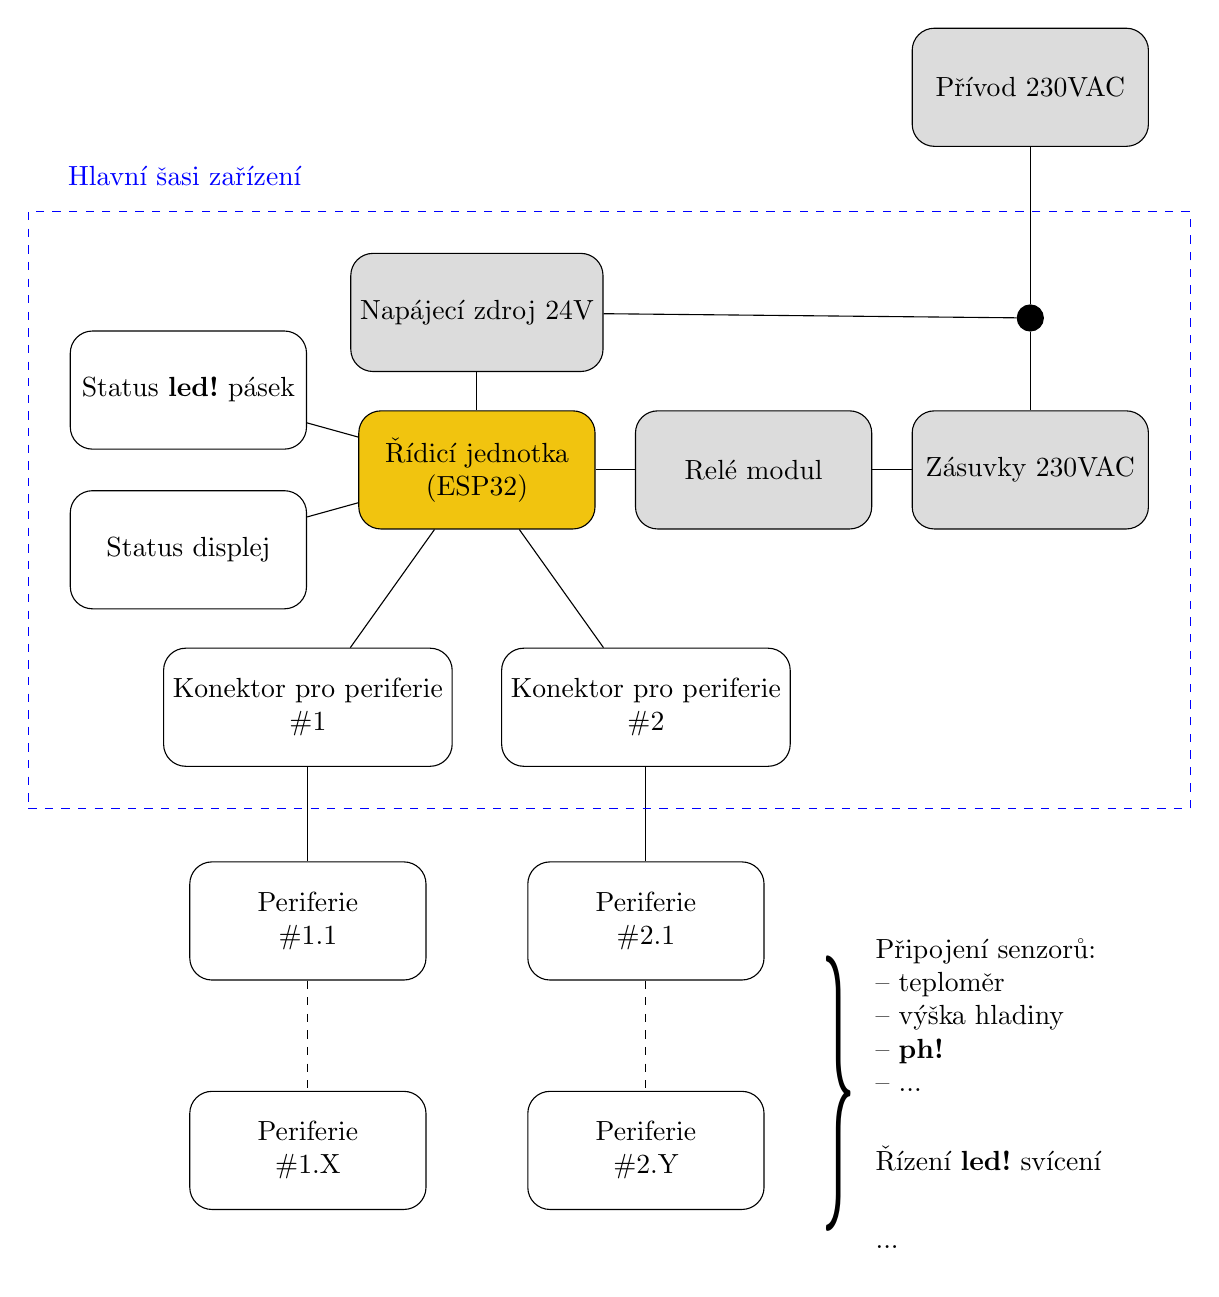
\begin{tikzpicture}[
            node distance=2cm,
            blok/.style={draw, rectangle, rounded corners=8pt, minimum height=1.5cm, minimum width=3cm},
            rect/.style={draw, dashed, blue, inner sep=15pt, fit=#1},
            label/.style={blue}
        ]
            % barvičky
            \definecolor{barva-silove}{RGB}{220, 220, 220}
            \definecolor{barva-ridici}{RGB}{241, 196, 15}
        
            \node (napajeni) [blok, fill=barva-silove] {Napájecí zdroj 24V};
            \node (ridici) [blok, below of = napajeni, align=center, fill=barva-ridici] {Řídicí jednotka \\ (ESP32)};
            \node (rele) [blok, right=0.5 of ridici, fill=barva-silove] {Relé modul};
            \node (zasuvky) [blok, right=0.5 of rele, fill=barva-silove] {Zásuvky 230VAC};
            \node (uzel) [style={draw, circle, minimum size=0.1cm, fill}, above=1cm of zasuvky] {};
            \node (sit) [blok, above= of uzel, fill=barva-silove ] {Přívod 230VAC};
            \node (display) [blok, below left=-0.5cm and 0.65cm of ridici] {Status displej};
            \node (ledstrip) [blok, above left=-0.5cm and 0.65cm of ridici] {Status \acs{led} pásek};

            \node (konektor1) [blok, align=center, below left=1.5cm and -1.2cm of ridici] {Konektor pro periferie \\ \#1};
            \node (konektor2) [blok, align=center, below right=1.5cm and -1.2cm of ridici] {Konektor pro periferie \\ \#2};

            % Periferie
            \node (per1-1) [blok, align=center, below=1.2cm of konektor1] {Periferie \\ \#1.1};
            \node (per1-x) [blok, align=center, below=1.4cm of per1-1] {Periferie \\ \#1.X};
        
            \node (per2-1) [blok, align=center, below=1.2cm of konektor2] {Periferie \\ \#2.1};
            \node (per2-y) [blok, align=center, below=1.4cm of per2-1] {Periferie \\ \#2.Y};

            % Popisek
            \node (vlastovka) [font=\fontsize{35}{14}\selectfont, yscale=4,  above right=-5.2cm and 0.6cm of per2-1] {\}}; 

            \node (popisek1) [right=0cm of vlastovka,yshift=1cm, align=left] {Připojení senzorů: \\ -- teploměr \\ -- výška hladiny \\ -- \acs{ph} \\ -- ...};
            \node (popisek2) [below=1cm of popisek1.south west, anchor=south west, align=left] {Řízení \acs{led} svícení};
            \node (popisek3) [below=1cm of popisek2.south west, anchor=south west, align=left] {...};

            % Spojovací linie
            \draw[-] (sit) -- (uzel);
            \draw[-] (uzel) -- (napajeni);
            \draw[-] (uzel) -- (zasuvky);
            \draw[-] (napajeni) -- (ridici);
            \draw[-] (ridici) -- (napajeni);
            \draw[-] (ridici) -- (display);
            \draw[-] (ridici) -- (ledstrip);
            \draw[-] (ridici) -- (konektor1);
            \draw[-] (ridici) -- (konektor2);
            \draw[-] (ridici) -- (rele);
            \draw[-] (rele) -- (zasuvky);
    
            \draw[-] (konektor1) -- (per1-1);
            \draw[dashed] (per1-1) -- (per1-x);
            
            \draw[-] (konektor2) -- (per2-1);
            \draw[dashed] (per2-1) -- (per2-y);
            
        
            % Obdélník, který obklopí vybrané uzly
            \node (hlavni-cast) [rect={(napajeni) (display) (ledstrip) (konektor1) (zasuvky)}] {};
            \node[label,above left=0.2cm and -3.6cm of hlavni-cast] {Hlavní šasi zařízení};
        \end{tikzpicture}
        
        \caption{Blokové schéma systému.}
        \label{fig:blokove-schema}
    \end{figure}
    
    Pro napájení vlastní elektroniky zařízení je v~šasi umístěn hotový modul spínaného zdroje převádějící síťové napětí \qty{230}{V} na stejnosměrných \qty{24}{V} se kterými pak zařízení dále pracuje (viz kapitola~\ref{sec:ridici-jendotka-napajeci-obvod}).   
    
    Z~hlediska bezpečnosti je potřeba zajistit, aby se uživatel ani samotná nízkonapěťová část obvodu nemohli dostat do kontaktu s~nebezpečným napětím. Toho je dosaženo galvanickým oddělením částí zařízení pracujících se síťovým napětím. V~blokovém schématu (obr.~\ref{fig:blokove-schema}) jsou všechny tyto části podbarveny šedou barvou. Pro spínaní síťových zásuvek jsou použita relé, která sama o sobě tvoří galvanickou izolaci, pro ještě lepší ochranu mikrokontroléru je pak zvolena varianta modulu obsahující také optočleny. Pro napájecí zdroj s~výstupem \qty{24}{V} je přítomnost galvanického oddělení kontrolována v~dokumentaci výrobce. 
    


    
    














\chapter{Návrh řídicí jednotky}
    Řídicí jednotka je jádrem celého zařízení. Její funkcí je řízení systému a zároveň komunikace s~uživatelem za pomoci Wi-Fi. Musí v~sobě nést informaci o~konfiguraci systému a na jejím základě zpracovávat data z~jednotlivých připojených periferií. Podle uživatelem nastavených scénářů pak dynamicky reaguje na změny hodnot měřených akvaristických veličin a ovládá akční členy (osvětlení, ohřev, filtr vody). Za pomoci displeje a \acs{led} pásku také informuje uživatele o~momentálním stavu zařízení. 

    \section{Mikrokontrolér}

    Při výběru vhodného mikrokontroléru bylo potřeba zohlednit výše zmíněné požadavky, tedy zejména Wi-Fi konektivitu a dostatečný výkon k~její obsluze, periferii \acs{can} a dostatek \acs{gpio} pinů pro připojení zbylých modulů v~hlavním šasi (viz obr.~\ref{fig:blokove-schema}). Na trhu existuje vícero výrobců nabízejících mikrokontroléry s~vhodnými parametry, z~důvodu jednoduchosti použití a nízké ceny byl nakonec zvolen model ESP32 od firmy Espressif, konkrétně modul WROOM-32E~\cite{esp32-wroom-32e-datasheet} s~čipem ESP32-D0WDR2-V3~\cite{esp32-datasheet}. Tento modul je často využíván v~různých hobby projektech, ale také v~komerčních aplikacích zejména v~oblasti chytré domácnosti. Z~tohoto důvodu k~němu existuje velká škála softwarových knihoven a v~rámci komunity uživatelů je také sdíleno mnoho projektů, kterými je možné se inspirovat.

    \clearpage
    \section{Návrh zapojení a tvorba \acs{dps}}
\label{sec:ridici-jednotka-schema-a-dps}
    Řídicí jednotka je tvořena jednou \acs{dps}, která kromě samotného mikrokontroléru obsahuje také měnič napětí typu buck ke snížení napájecího napětí externího zdroje na hodnotu \qty{5.2}{V}. Toto napětí je pak dále používáno pro napájení samotného mikrokontroléru řídicí jednotky a zároveň je vyvedeno na konektor pro připojení periferií. Blokové schéma na úrovni logických bloků v~rámci jedné \acs{dps} je na obr.~\ref{fig:ridici-jednotka-blokove-schema}, jednotlivým částem se blíže věnují další kapitoly. Celé schéma je k~dispozici v~příloze~\ref{priloha:schema-a-dps-ridici-jednotka}.

    % Blokove schema
    \begin{figure}[h!]
        \centering
        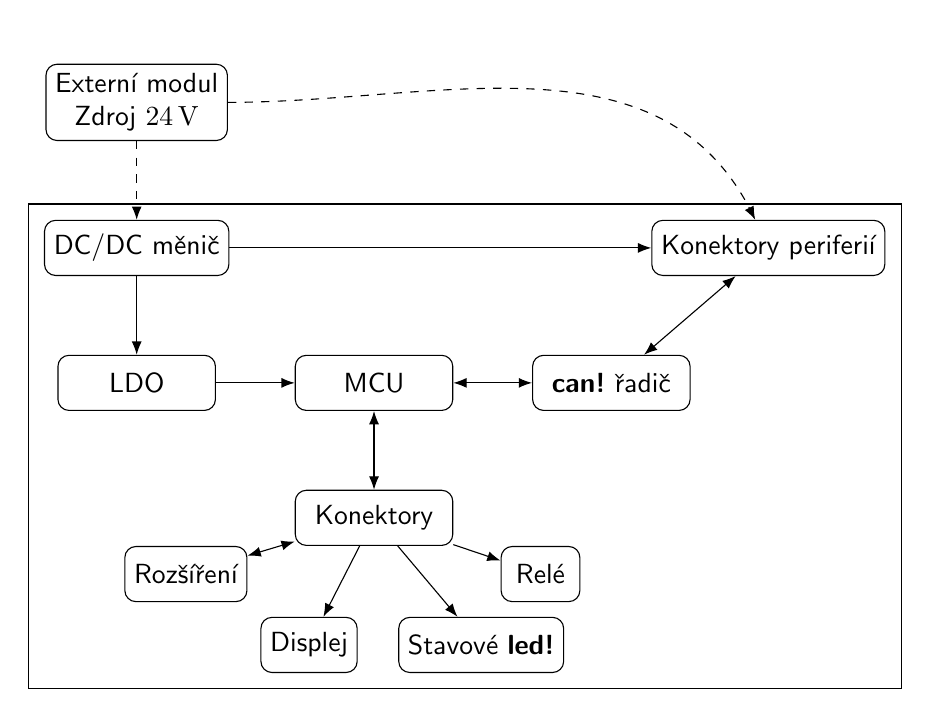
\begin{tikzpicture}[
            module/.style={%
        draw, rounded corners,
        minimum width=#1,
        minimum height=7mm,
        font=\sffamily,
        align=center
        },
    module/.default=2cm,
    >=LaTeX]
        
            % ridici
            \node[module] (mcu) {MCU};
            \node[module, left=of mcu] (ldo) {LDO}; 
            \node[module, above=of ldo] (buck) {DC/DC měnič};
            \node[module, right=of mcu] (candriver) {\acs{can} řadič};
            \node[module, above right=10mm and -5mm of candriver] (konperif) {Konektory periferií};
            \node[module, above=of buck] (24v) {Externí modul\\Zdroj \qty{24}{V}};
            \node[module, below=of mcu] (konektory) {Konektory};
            \node[module=1cm, below right=9mm and -7mm of konektory] (konektor1) {Stavové \acs{led}};
            \node[module=1cm, below left= 9mm and -8mm of konektory] (konektor2) {Displej};
            \node[module=1cm, below right= 0mm and 6mm of konektory] (konektor3) {Relé};
            \node[module=1cm, below left= 0mm and 6mm of konektory] (konektor4) {Rozšíření};

            \node[fit=(konektor1) (konektor2) (konektor3) (konektor4) (buck) (konperif) (mcu), draw, inner sep=2mm] (fitridici) {};
            % Connections
            \foreach \i in {1,2,3}
                \draw[->] (konektory)--(konektor\i);
            \draw[<->] (konektory)--(konektor4);
            \draw[<->] (konektory)--(mcu);
            \draw[->] (buck)--(ldo);
            \draw[->] (ldo)--(mcu);
            \draw[<->] (candriver)--(mcu);
            \draw[->] (buck)--(konperif);
            \draw[<->] (candriver)--(konperif);

            \draw[->,dashed] (24v) to [out=0,in=115] (konperif);
            \draw[->,dashed] (24v)--(buck);
        
        \end{tikzpicture}
        
        \caption{Blokové schéma řídicí jednotky.}
        \label{fig:ridici-jednotka-blokove-schema}
    \end{figure}

    \subsection{Zapojení ESP32 modulu}
    \label{sec:ridici-jendotka-esp32-modul}
        Při tvorbě schématu bylo vycházeno z~dokumentace výrobce~\cite{esp32-wroom-32e-datasheet} a také ze schémat různých existujících vývojových desek. K~zajištění správné a spolehlivé funkce modulu je potřeba dodržet několik věcí. Výřez schématu obsahující potřebné doplňující obvody pro ESP32 modul je na obr.~\ref{fig:ridici-jednotka-esp-obvody}.

        \begin{figure}[h!]
            \centering
            % trim=left bottom right top
            \includegraphics
            [
                width=0.9\textwidth, 
                page=2, 
                trim=2.5cm 8.5cm 15.5cm 2cm, 
                clip
            ]{obrazky/exportovane/main-board-schematic.pdf}
            \caption{Podpůrné obvody pro modul ESP32-WROOM-E. Vytvořeno v~KiCad 7.0.}
            \label{fig:ridici-jednotka-esp-obvody}
        \end{figure}

        Na napájecí pin (3V3) je třeba přivést stabilní napětí a opatřit ho blokovacími kondenzátory (C3, C4). Ke snížení napětí z~původních \qty{5,2}{V} na požadovaných \qty{3,3}{V} je použit lineární regulátor TLV76133 (U2).
        
        % TODO: Čas ke stabilizaci bude mnohem větší než 50 us. Nejprve totiž musí naběhnout 3V3, což trvá dle datasheetu TLV76133 trvá cca 500 us. Taky bys správně měl zohlednit i náběh 5V2, což je 3 ms.
        Dále je potřeba přivést kladné napětí na povolovací pin (EN). Z~dokumentace vyplývá, že by mělo být přivedeno až po ustálení napájecí linky. Uvedený čas nutný ke stabilizaci je roven \(t_{STBL}=\qty{50}{\micro\second}\)~\cite{esp32-datasheet}. Požadované zpoždění zajistí RC článek (R1, C5) s~časovou konstantou \(\tau\):
        \begin{equation}
            \tau=R_{1}C_{5}=\qty{10}{\kilo\ohm}\cdot \qty{1}{\micro\farad}=\qty{10}{\milli\second}
        \end{equation} 
        Jak je vidět, byla zvolena dostatečná návrhová rezerva. 

        Pro možnost resetu zařízení a vstupu do bootloaderu byla doplněna také dvě tlačítka (SW1, SW2).



    \subsection{Napájecí obvod}
        \label{sec:ridici-jendotka-napajeci-obvod}
        Pro napájení celého zařízení je použit externí zdroj stejnosměrného napětí \qty{24}{V} a toto napětí je také rozvedeno všem připojeným periferiím. Pro většinu komponent je ale nutné napětí snížit. K~tomuto účelu byl navržen DC/DC měnič typu buck s~požadovaným výstupním napětím \qty{5.2}{V}. Existuje celá řada čipů vyvinutých pro tento účel. Aplikace v~tomto zařízení je specifická svými požadavky na výstupní proud. Zatímco samotná řídicí jednotka nebude odebírat velký proud, není jasně dané, kolik periferí a s~jakými výkonovými požadavky uživatel k~systému připojí. Navržený měnič tak musí fungovat v~širším rozsahu proudů (řádově od desítek mA po jednotky A), a to s~co nejlepší účinností. 
        
        \begin{figure}[h!]
            \centering
            % trim=left bottom right top
            \includegraphics
            [
                width=\textwidth, 
                page=2, 
                trim=2.2cm 8.5cm 13cm 1.3cm, 
                clip
            ]{obrazky/exportovane/ukazky-do-textu.pdf}
            \caption{Napájecí obvod řídicí jednotky. Vytvořeno v~KiCad 7.0.}
            \label{fig:ridici-jednotka-napajeni-simp}
        \end{figure}

        
        Aby bylo vyhověno zmíněným požadavkům a zachována návrhová rezerva, byl jako základ buck měniče zvolen čip LM5148~\cite{lm5148-datasheet}. Jedná se o~moderní součástku firmy Texas Instruments s~velkou výkonovou rezervou. Tento čip funguje pouze jako buck kontrolér a zapojení je potřeba doplnit dvěma externími MOSFET tranzistory. Většina tepelných ztrát vzniká právě na nich, čímž se sníží ohřev samotného čipu a generované teplo se lépe rozloží. Na volbě tranzistorů závisí také výsledná účinnost měniče. Při návrhu zapojení této součástky byl použit nástroj Webench Power Designer~\cite{webench-power-designer}, který podle zadaných parametrů navrhne konkrétní schéma zapojení, provede simulaci a zobrazí grafy upravené na míru zadaným hodnotám. Tento nástroj uvádí přibližnou účinnost zapojení jako \qty{88}{\percent}. V~navrženém schématu bylo posléze provedeno několik změn, aby vše odpovídalo požadavkům uvedeným v~katalogovém listu součástky~\cite{lm5148-datasheet}. Kompletní schéma zapojení spolu s odkazy k relevantním kapitolám katalogového listu se nachází v příloze~\ref{priloha:schema-ridici-jednotka-napajeci-obvod}, pro přibližnou představu pak postačí zjednodušené schéma na obr.~\ref{fig:ridici-jednotka-napajeni-simp}. 

        \textit{TODO: výpočty by asi bylo dobré uvést co?}

    \subsection{Deska plošných spojů}
        Ačkoliv se jedná o relativně jednoduchou \acs{dps}, je potřeba při návrhu dbát jistých pravidel a doporučení. Modul ESP32 je vybaven anténou a volba jeho umístění na \acs{dps} je rozhodujícím faktorem pro správnou funkci antény. Další částí vyžadující optimální návrh rozložení a propojení součástek je pak buck měnič. 
        
        \begin{figure}[!ht]
            \centering
            \begin{tikzpicture}
                % Include the image
                \node[anchor=south west,inner sep=0] (image) at (0,0) {\includegraphics[width=0.8\textwidth]{obrazky/dps/mainBoard-3d-top-popis.png}};
                
                % \draw[->,thick] (0,0) -- (1,9.4);
                \node[anchor=south west,inner sep=0,color=red] at (0.5,9.7)  {1.};
                \node[anchor=south west,inner sep=0,color=red] at (0.6,1.3)  {2.};
                \node[anchor=south west,inner sep=0,color=red] at (4.2,-0.4)  {3.};
                \node[anchor=south west,inner sep=0,color=red] at (6.8,1.3)  {4.};
                \node[anchor=south west,inner sep=0,color=red] at (6.8,5)  {5.};
                % legend
                \node[anchor=south west,inner sep=0] (leg-blu) at (8.5,10)  {\acs{mcu}};
                \node[anchor=south west,inner sep=0] (leg-ora) at (8.5,9.32) {buck měnič napětí};
                \node[anchor=south west,inner sep=0] (leg-red) at (8.5,8.64) {Konektory:};

                \node[below left=0.8 and 0.6 of leg-red, anchor=south west] (kon1) {1. Ovládané periferie};
                \node[below left=0.6 and 0.0 of kon1, anchor=south west] (kon2) {2. Externí moduly};
                \node[below left=0.6 and 0.0 of kon2, anchor=south west] (kon3) {3. Programování};
                \node[below left=0.6 and 0.0 of kon3, anchor=south west] (kon4) {4. Vstup napájení};
                \node[below left=0.6 and 0.0 of kon4, anchor=south west] (kon5) {5. Testování, rozšíření};
                % \node[anchor=south west,inner sep=0,color=red] {2.};
                % \node[anchor=south west,inner sep=0,color=red] {3.};
                % \node[anchor=south west,inner sep=0,color=red] {4.};
                % \node[anchor=south west,inner sep=0,color=red]          {5.};
            \end{tikzpicture}
            \caption{Vizualizace \acs{dps} řídicí jednotky s vyznačením jednotlivých částí.}
            \label{fig:ridici-jednotka-dps-popis}
        \end{figure}

        Prvním krokem návrhu je volba počtu vrstev a jejich funkce. Vyšší počet vrstev nabízí více prostoru pro vedení cest a také umožňuje vedení napájecích napětí pomocí rozlitých měděných polygonů, čímž se zároveň zlepší vlastnosti zařízení z hlediska \acs{EMC}. Zvolený výrobce (JLC PCB~\cite{jlcpcb}) nabízí výrobu desek s jednou až dvaceti vrstvami mědi. Byla zvolena čtyřvrstvá deska, která je pro danou aplikaci dostatečná a stále se nachází v přijatelné cenové skupině výrobce. Rozložení a funkce vrstev jsou vyobrazeny na obr.~\ref{fig:ridici-jednotka-stackup-dps}.

        Pro optimální fukci Wi-Fi antény výrobce doporučuje umístit ESP32 modul do pravého horního rohu \acs{dps} tak, aby se pod anténou nenacházela vrsta mědi a nejlépe ani samotná deska~\cite{esp32-hw-guidelines}. Na obr.~\ref{fig:ridici-jednotka-dps-popis} je zobrazen výsledný návrh \acs{dps}, kde v modře vyznačené oblasti lze vidět, že tyto požadavky byly splněny. Vedle ESP32 modulu se nachází související součástky popsané v kapitole~\ref{sec:ridici-jendotka-esp32-modul}.

        \begin{figure}[h!]
            \centering
            % trim=left bottom right top
            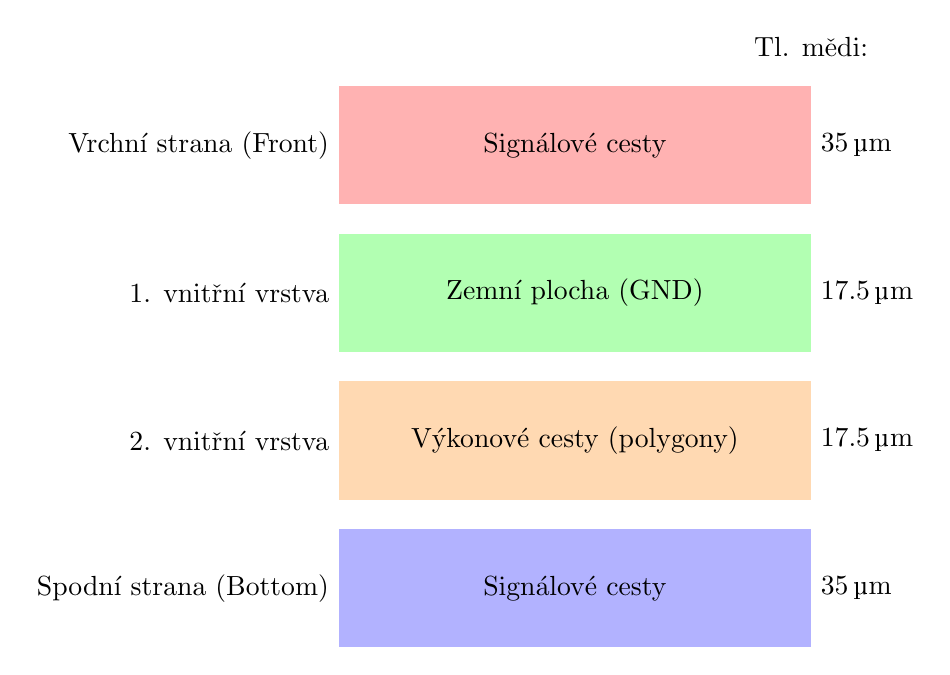
\begin{tikzpicture}[scale=1.5]

                % Layers
                \fill[red!30]    (0,3.75)   rectangle (4,4.75);
                \fill[green!30]  (0,2.5)    rectangle (4,3.5);
                \fill[orange!30] (0,1.25)   rectangle (4,2.25);
                \fill[blue!30]   (0,0)      rectangle (4,1);
                

                % Layer labels
                \node at (2,4.25) {Signálové cesty};
                \node at (2,3) {Zemní plocha (GND)};
                \node at (2,1.75) {Výkonové cesty (polygony)};
                \node at (2,0.5) {Signálové cesty};

                \node[anchor=east] at (0,4.25) {Vrchní strana (Front)};
                \node[anchor=east] at (0,3)    {1. vnitřní vrstva};
                \node[anchor=east] at (0,1.75) {2. vnitřní vrstva};
                \node[anchor=east] at (0,0.5)  {Spodní strana (Bottom)};

                \node[anchor=north] at (4,5.25) {Tl. mědi:};
                \node[anchor=west] at (4,4.25) {\qty{35}{\micro m}};
                \node[anchor=west] at (4,3)    {\qty{17.5}{\micro m}};
                \node[anchor=west] at (4,1.75) {\qty{17.5}{\micro m}};
                \node[anchor=west] at (4,0.5)  {\qty{35}{\micro m}};
                
                % Comments
                % \draw[<-,thick] (0,3.75)    -- +(0.5,-0.5) node[below] {Bottom Layer};
                % \draw[<-,thick] (0,2.5)     -- +(0.5,-0.5) node[below] {Inner Layer 2};
                % \draw[<-,thick] (0,1.25)    -- +(0.5,-0.5) node[below] {Inner Layer 1};
                % \draw[<-,thick] (0,0)       -- +(0.5,-0.5) node[below] {Top Layer};
                
                \end{tikzpicture}
            \caption{Rozložení vrstev \acs{dps} řídicí jednotky.}
            \label{fig:ridici-jednotka-stackup-dps}
        \end{figure}


        \subsubsection{Měnič napětí}
            \textit{TODO: Zde popis návrhu, zdroje, obrázky}
            \textit{Q: Jak moc do detailu?}

   

    \section{Konektivita}
        Řídicí jednotka je vybavena několika konektory, jak je opět možno vidět na obr.~\ref{fig:ridici-jednotka-dps-popis}. Na levé straně \acs{dps} (značeno 1.) se nachází konektory pro připojení periferií připravené pro montáž do panelu, kde pak budou přístupné uživateli. Ostatní vyznačené konektory slouží pro připojení externích modulů v rámci hlavního šasi (viz blokové schéma na obr.~\ref{fig:blokove-schema}) popř. pro programování a testování, nebudou tedy volně přístupné uživateli.

        Abychom předešli poškození zařízení při nevhodném zacházení uživatelem, je potřeba pro volně dostupné konektory přidat dodatečnou ochranu~\cite{altium-circuit-protection}. Jak je vidět na obr.~\ref{fig:komunikacni-rozhr-dsub-pinout}, konektor pro periferie sdružuje jak datovou komunikaci, tak i napájení. Ochranu diferenční datové linky zajistí samotný \acs{can} řadič, který je určen pro průmyslové použití a obsahuje zabudovanou ochranu jak proti zkratu datové linky s napájením či zemí, tak proti ESD~\cite{ata-datasheet}. 

        \begin{figure}[h!]
            \centering
            % trim=left bottom right top
            \includegraphics
            [
                width=0.9\textwidth, 
                page=5, 
                trim=8.5cm 7.6cm 7.5cm 3cm, 
                clip
            ]{obrazky/exportovane/main-board-schematic.pdf}
            \caption{Zapojení a ochrana konektorů. Vytvořeno v~KiCad 7.0.}
            \label{fig:ridici-jednotka-konektory}
        \end{figure}

        Co se týče napájecích vodičů, každý z nich je ošetřen vratnou pojistkou (ang. polyfuse) dimenzovanou podle předpokládaného maximálního odběru zařízení. Při překročení tohoto proudu, např. z důvodu zkratu v některé z periferií, pojistka sepne a proud v obvodu omezí na minimum. Schéma zapojení konektorů spolu s hodnotami vratných pojistek se nachází na obr.~\ref{fig:ridici-jednotka-konektory}.


            
    

            

\chapter{Obecný modul periferie}
    Díky zvolené koncepci systému je možné za periferii považovat jakékoliv zařízení schopné obousměrně komunikovat po navržené sběrnici. Není vyloučeno, aby byla každá periferie navržena zcela odlišně na základě svých vlastních požadavků na výkon, počet pinů nebo dostupná rozhraní daného MCU. Hlavní výhodou této koncepce je to, že periferie mohou být vyvíjeny postupně a přidávány do již funkčního a odladěného systému bez nutnosti modifikovat stávájící hardware. V~případě chyby v~návrhu periferie je také oprava méně náročná, než by tomu bylo v~případě zabudování veškeré funkcionality přímo do řídící jednotky. 

    Nicméně pokud by byl pro každou periferii zvolen zcela jiný mikrokontroler a vytvořen vlastní návrh DPS, vývoj více periferií by byl zbytečně drahý a časově náročný. Proto byl zvolen koncept \uv{obecného modulu periferie}, tedy jedné DPS s~konkrétním mikrokontrolerem zajišťující připojení ke komunikačního rozhraní, napájení periferie a rozhraní pro programování. Kromě toho budou na DPS dvě dutinkové lišty, do kterých bude možné vsadit druhou DPS (popř. během vývoje pouze prototypovací desku) ve funkci dceřinné desky (ang. daughterboard). Vložená deska pak bude obsahovat obvody nutné přímo pro danou konkrétní periferii.
    
    \section{Mikrokontrolér}

        Kritéria pro výběr mikrokontroleru byla následující:
        \begin{itemize}
            \item Musí nutně splňovat:
            \begin{itemize}
                \item CAN periferie -- pro komunikaci po sběrnici 
                \item PWM výstup -- řízení LED, popř. jiné
                \item ADC -- pro práci s analogovými sensory
                \item Nízká cena 
            \end{itemize}
            \item Je výhodou:
            \begin{itemize}
                \item Dobrá dokumentace, komunita uživatelů
                \item Zkušenost autora s~danou platformou
                \item Další periferie (\acs{i2c}, SPI, ...)
            \end{itemize}
        \end{itemize}

        Na základě těchto kritérií byl vybrán mikrokontroler \textbf{PIC16F15325} od firmy Microchip, ten splňuje všechna kritéria a disponuje také množstvím dalších periferií, které by mohly být v~budoucnu užitečné~\cite{PIC18F26Q83}.

    \section{Návrh zapojení a tvorba DPS}
        Celé schéma pro obecný modul periferie se nachází v příloze~\ref{TODO}. Návrh zapojení lze rozdělit na tři části. V prvním kroku je zapojen mikrokontroler tak, aby byly opět splněny všechny požadavky výrobce. Mikrokontrolery řady PIC se vyznačují značnou jednoduchostí použití a ke správnému chodu jim stačí jen minimum dalších součástek. V případě PIC18F26Q83 postačí připojit blokovací kondenzátor (C6) na napájení (pin VCC) a přivést kladné napětí na resetovací pin (MCLR). MCU je dále doplněn resetovacím tlačítkem pro pohodlnější práci při vývoji a testování firmwaru a regulátorem napětí (U1) s výstupem \qty{3.3}{V}. 

        Ve druhém kroku je přidána dvojice D'sub konektorů a CAN řadič ATA6561 obdobně jako u řídící jednotky popsané v sekci \ref{sec:ridici-jednotka-schema-a-dps}. Na závěr jsou všechny dosud nevyužité piny vyvedeny na konektor (dutinkovou lištu), aby byly jednoduše dostupné pro připojenou dceřinnou desku. Pro napájení výkonově náročnejších periferií (např. ovladač LED osvětlení) jsou zvlášť vyvedeny ještě dvě trojice pinů připojené na \qty{24}{V} a zem (GND).

        \subsubsection{Tvorba DPS}
        Hlavním cílem bylo vytvořit DPS co nejmenší, jelikož se jedná o samostatné moduly, kterých bude v systému zapojeno několik a pro manipulaci a rozmístění modulů okolo akvária je menší rozměr výhodou. Hlavní limitací v této snaze není počet součástek, ale spíše rozměry mechanických prvků, zejména konektorů D'sub. Na obr.~\ref{fig:modul-periferie-dps} je vidět výsledný návrh DPS s osazenými součástkami a dosaženými rozměry. Je zřejmé že jiným rozložením dutinkových lišt by se návrh dal ještě drobně zmenšit, ale je potřeba ponechat jistou flexilitu pro tvorbu dceřinných desek.

        \begin{figure}[!ht]
            \centering
            \begin{tikzpicture}
                % Include the image
                \node[anchor=south west,inner sep=0] (image) at (0,0) {\includegraphics[width=0.8\textwidth]{obrazky/dps/peripherial-module-3d-top.png}};
                
                \draw[dashed] (10.1,0.04) -- (12.5,0.04);
                \draw[<->,thick] (12.5,0.04) -- (12.5,6.34);
                \draw[dashed] (12.5,6.34) -- (10.1,6.34);
                \node[anchor=west] at (12.5,3.15)  {\qty{36}{mm}};

                \draw[dashed] (1.12,0.64) -- (1.12,-0.5);
                \draw[<->,thick] (1.12,-0.6) -- (10.9,-0.6);
                \draw[dashed] (10.9,-0.6) -- (10.9,0.64);
                \node[anchor=south] at (6,-0.6)  {\qty{57}{mm}};
            \end{tikzpicture}
            \caption{Vizualizace DPS obecného modulu periferie.}
            \label{fig:modul-periferie-dps}
        \end{figure}

        Co se týče rozložení vrstev, byla opět použita čtyřvrstvá deska se strejnou strukturou jako je na obr.~\ref{fig:ridici-jednotka-stackup-dps} pro DPS řídící jednotky. Celý návrh DPS se nachází v příloze TODO.





\chapter{Volba a návrh periferií}
    Tato kapitola se již věnuje návrhu konkrétních periferií, tedy jednotlivých senzorů a akčních členů. Po technické stránce jsou všechny zmíněné moduly nadstavbou pro \uv{obecný modul periferie} popsaný detailně v předešlé kapitole. Jelikož je celý systém modulární, je pravděpodobné, že postupem času bude dále rozšiřován o nové typy periferií a i v současné chvíli je jich v plánu více, než je v možnostech této práce. Pro lepší přehlednost se v tab.~\ref{tab:prehled-periferii} nachází přehled všech realizovaných i v tuto chvíli pouze plánovaných periferií.

    \begin{table}[h]
        \centering
        \caption{Přehled periferií.}
        \label{tab:prehled-periferii}
        \begin{tabular}{|l|l|l|l|l|}
            \hline
            Název & Typ & Napájení & Funkce & Realizováno \\ \hline\hline
            Sensor teploty  & S & \qty{5}{V}    & Teplota vody                       & Ano, kap.~\ref{sec:perif-sensor-teploty}  \\ \hline
            Sensor hladiny  & S & \qty{5}{V}    & Výška hladiny (spojitě + skokově)  & Ano, kap.~\ref{sec:perif-sensor-hladina}  \\ \hline
            \acs{led} osvětlení   & A & \qty{24}{V}   & Intenzita osvětlení                & Ano, kap.~\ref{sec:perif-led-osvetleni}  \\ \hline
            Sensor \acs{ph}       & S & \qty{5}{V}    & \acs{ph} vody                            & Ano, kap.~\ref{sec:perif-sensor-ph}  \\ \hline
            Topné těleso    & A & \qty{230}{V}  & Ohřev vody                         & Ano, kap.~\ref{sec:perif-230v}  \\ \hline
            Filtr vody      & S & \qty{230}{V}  & Filtrace vody                      & Ano, kap.~\ref{sec:perif-230v}  \\ \hline
            Krmítko         & A & \qty{24}{V}   & Dávkování krmiva                   & Ne  \\ \hline
            Sensor průtoku  & S & -             & Voda tekoucí filtrem               & Ne  \\ \hline
                            % & S &  &  & A  \\ \hline
                            %     & S &  &  & A  \\ \hline
                            %     & S &  &  & A  \\ \hline
                            %     & S &  &  & A  \\ \hline
                            %     & S &  &  & A  \\ \hline
                            %     & S &  &  & A  \\ \hline
                            %     & S &  &  & A  \\ \hline
                            %     & S &  &  & A  \\ \hline
                            %     & S &  &  & A  \\ \hline
            \end{tabular}
            \begin{tabular}{c}
                S = sensor, A = akční člen \\
            \end{tabular}
   
    \end{table}

\section{\acs{led} osvětlení}
\label{sec:perif-led-osvetleni}

    Úkolem této periferie je zajistit osvětlení akvária a umožnit jeho ovládání. V porovnání s ostatními moduly je zapojení relativně komplexní a proto byla pro tuto periferii navržena a zhotovena vlastní \acs{dps} (fungující jako dceřinná deska, viz.~\ref{sec:modul-periferie}). Jako typ svítidla byly zvoleny \acs{led} pásky pracující s napětím \qty{12}{V}. Modul musí být schopen samostatně ovládat 2 \acs{led} pásky, kdy za pomocí regulace proudu do \acs{led} pásku nastaví intenzitu osvětlení. 

\subsection{Návrh zapojení}
    Na začátku návrhu je potřeba specifikovat si požadavky na elektrické parametry zapojení. Uvažujme délku každého pásku \(l=\qty{1}{m}\), vstupní napětí získané z konektoru D-sub \(U_{in} =\qty{24}{V}\) a výstupní napětí pro které je pásek určen \(U_{out} =\qty{12}{V}\). Pro stanovení maximálního proudu bylo vycházeno z údajů na e-shopu \acs{led} Solution~\cite{eshop-ledsolution-svetlo}, kdy nejvýkonější nabízený \acs{led} pásek pro dané napětí má příkon \(P_{i}= \qty{20}{W/m}\). Pak každý kanál musí být schopen dodat proud odpovídající nejnáročnějšímu scéáři:
    \begin{equation}  
        I_{max} = \frac{P_{i}\cdot l }{U_{out}} = \frac{20\cdot 1 }{12} = \qty{1.66}{A}
    \end{equation}

    Jelikož se jedná o dceřinnou desku pro obecný modul, rozměr výsledné \acs{dps} je omezen a část plochy je navíc využita konektory pro vsazení do obecného modulu. Je tedy potřeba zvolit co nejvíce integrované řešení, které současně slibuje dobrou účinnost a tedy co nejnižší ohřev zařízení během provozu.

    Pro řízení \acs{led} osvětlení je často používán proudový zdroj, který umožňuje lineárně regulovat výstupní proud a tím i intenzitu osvětlení. Na trhu existuje opět celá řada čipů určena přímo k ovládání \acs{led} pásků~\cite{TI_\acs{led}_Drivers}, problém je zde ale v tom, že uživatel velmi pravděpodobně připojí pásek s nižším, předem neznámým příkonem. Maximální proud je tedy specifický danému \acs{led} pásku a proudový zdroj by musel zároveň spolehlivě zaručit, že nebude překročeno napětí \(U_{out} =\qty{12}{V} \).

    Touto funkcí většina čipů nedisponuje a pokud ano, nejsou dostatečně integrované pro použití v této aplikaci. Po důkladné rešerši a několika iteracích návrhu se nakonec jeví jako nejlepší použití napěťového měniče typu buck spolu se zesilovačem pro snímání proudu. Snímaný proud je následně zpracován mikrokontrolérem a jsou upraveny poměry ve zpětné vazbě měniče, aby napětí odpovídalo požadovanému proudu.

    \begin{figure}[h!]
        \centering
        % trim=left bottom right top
        \includegraphics
        [
            width=\textwidth, 
            page=1, 
            trim=2.5cm 11.5cm 16cm 1.5cm, 
            clip
        ]{obrazky/exportovane/ukazky-do-textu.pdf}
        \caption{Zjednodušené schéma ovladače \acs{led}. Vytvořeno v~KiCad 7.0.}
        \label{fig:led-board-simp-schema}
    \end{figure}

    
\subsubsection{Popis schématu a výpočty hodnot součástek}
% TODO: projet ještě jednou poznámky od Pavla
    Zjednodušené schéma pro jeden ovládaný kanál se nachází na obr.~\ref{fig:led-board-simp-schema}, při výpočtech bude použito označení součástek z tohoto schématu. Úplné schéma modulu pak lze nalézt v příloze~\ref{priloha:schema-led-board}.

    Jako buck kontrolér je zvolen čip AP63356Q vyvinutý společností Diodes incorporated, jedná se o úspornou a velmi malou součástku, která v sobě integruje oba potřebné MOSFET tranzistory a spíná s pevně danou frekvencí \(f_{SW}=\qty{450}{kHz} \) ~\cite{Diodes_AP63356Q}. Pro snímání proudu poslouží čip INA180A4 firmy Texas Instruments~\cite{TI_INA180A4}.

    Z obrázku je vidět, že pro ovládání jednoho kanálu \acs{led} pásků jsou využity 4 piny \acs{mcu}, RA4 a RB1 fungují jako vstupy, RA2 a RA3 pak jako výstupy. Rezistor \(R_{1}\) drží buck měnič ve vypnutém stavu dokud mikrokontrolér nenastaví hodnotu pinu RA2 na logickou 1. Pin RA4 je pak čipem (U1) stažen k zemi vždy, když na výstupu není odpovídající nastavené napětí.  
    
    Nastavení výstupního napětí měniče je dosaženo za pomoci zpětnovazební smyčky mezi výstupním uzlem (I.) a zpětnovazebním pinem FB (uzel II.). V uzlu II. je drženo konstantní napětí \qty{0.8}{V}~\cite{Diodes_AP63356Q}, poměrem rezistorů R3 a R4 je pak definováno výstupní napětí. Zvolíme hodnotu odporu \(R_{4} = \qty{10}{k\ohm}\), pro maximální požadované napětí \(U_{outMAX} = \qty{12}{V}\) platí:
    \begin{equation}
        R_{3} = R_{4}\cdot \left(\frac{U_{outMAX} }{\num{0.8}}-1\right) = \qty{10}{k}\cdot \left(\frac{12}{\num{0.8}}-1\right) = \qty{140}{k\ohm}
    \end{equation} 
    Na pin RA3 mikrokontroléru je přivedeno analogové napětí z periferie \acs{dac} popř. \acs{pwm} signál a skrze rezistor R5 (a ochrannou diodu) pak teče proud do rezistoru R4, úbytek napětí na tomto rezistoru je ale konstantní (\qty{0.8}{V}) a tedy je konstantní i proud rezistorem. Z prvního Kirchhoffova zákona pak víme, že proud rezistorem R3 klesne o hodnotu proudu dodanou z pinu RA3, tím klesne také napětí na výstupu měniče a dojde ke ztlumení jasu \acs{led} pásku. Citlivost (nebo také rozsah) změny je definován hodnotou R5, snížením jeho hodnoty lze dosáhnout na výstupu ještě nižšího napětí. Pro hodnotu \(R_{5} = \qty{100}{k\ohm}\) zobrazenou ve schématu lze nejnižší možné napětí vypočítat následovně:
    \begin{equation}
        U_{outMIN} = \num{0.8}+R_{3} \cdot I_{3} = \num{0.8}+R_{3} \cdot \left(\frac{\num{0.8}}{R_{4}} - \frac{U_{VDD} - U_{D1}}{R_{4}+R_{5}} \right) 
    \end{equation}  
    Kdy \(U_{VDD} = \qty{3.3}{V}\) je maximální napetí pinu RA3 a \(U_{D1}=\qty{0.35}{V} \) je prahové napětí zvolené diody. Po dosazení získáme:
    \begin{equation}
        U_{outMIN} = \num{0.8}+\qty{140}{k} \cdot \left(\frac{\num{0.8}}{\qty{10}{k}} - \frac{\num{3.3} - \num{0.35}}{\qty{10}{k}+\qty{100}{k}} \right) = \qty{8.25}{V}
    \end{equation}  
    Toto napětí by mělo být dostatečně nízké k úplnému zhasnutí \acs{led} pásku.

    TODO: Kompenzace

    V dalším kroku je stanovena hodnota induktoru L1. Výrobce doporučuje zvolit zvlnění proudu induktorem (ripple) \(\Delta I_{L}  \) jako 30 až \qty{50}{\percent} maximálního proudu čipu. Při zvolení střední hodnoty \qty{40}{\percent} získáme:
    \begin{equation}
        \Delta I_{L} = \num{0.4}\cdot I_{IC-max} = \num{0.4} \cdot  \num{3.5} = \qty{1.4}{A}
    \end{equation}
    Odpovídající hodnota indukčnosti je vypočtena následujícím vztahem:
    \begin{equation}
        L_{1} = \frac{U_{outMAX}\cdot (U_{in} -U_{outMAX} ) }{U_{in} \cdot \Delta I_{L}\cdot f_{SW}  }
    \end{equation}
    Po dosazení získáme:
    \begin{equation}
        L_{1} = \frac{12\cdot (24 -12 ) }{24 \cdot \num{1.4}\cdot \qty{450}{k}  } = \qty{9.52}{\micro H}
    \end{equation}
    Zvolíme nejbližší běžně používanou hodnotu \(L_{1} = \qty{10}{\micro H}\).

    Pro vstupní (C1) a výstupní (C6) kapacitu použijeme hodnoty doporučené výrobcem, stejně tak pro bootstrap kondenzátor C3. 
    
    Poslední součástkou zůstává měřicí rezistor R6. Tímto rezistorem protéká celý výstupní proud měniče, v rámci minimalizace ztrátového výkonu by měl mít tedy co nejmenší odpor. Musíme ovšem také brát v potaz rozsah měřicího zesilovače INA180A4. Tato součástka se vyrábí v několika variantách, byla zvolena varianta s nejvyšším ziskem \(G_{INA}=200 \) pro zachování co nejnižší hodnoty rezistoru, výstupní napětí zesilovače je v rozsahu 0 až \qty{3.3}{V} (VDD mikrokontroléru).
    Při maximálním očekávaném proudu chceme dosáhnout horní hranice rozsahu zesilovače, z této podmínky vyplývá vztah pro výpočet odporu rezirtoru R6:
    \begin{equation}
        R_{6} = \frac{U_{VDD}}{I_{max} \cdot G_{INA} } = \frac{\num{3.3}}{\num{1.66}\cdot 200} = \qty{9.94}{m\ohm}
    \end{equation} 
    Zvolíme blízkou hodnotu \(R_{6} \) = \qty{10}{m\ohm}.


\subsubsection{Očekávané parametry}
    Pro výpočet výstupního zvlnění (v uzlu I.) chybí údaj o ekvivalentním sériovém odporu (ESR) výstupních kondenzátorů (C6), který výrobce neuvádí. Vyjdeme tedy z typické hodnoty pro keramický kondenzátor \(ESR=\qty{15}{m\ohm}\)~\cite{wikipedia2024esr}, kdy počítáme s paralelní kombinací tří kondenzátorů.
    Očekávané výstupní zvlnění je tedy přibližně:
    \begin{equation}
        \Delta U_{out} = \Delta I_{L} \cdot  \left(\frac{ESR}{3}+\frac{1}{8\cdot f_{SW} \cdot C_{6} }\right) 
    \end{equation} 
    \begin{equation}
        \Delta U_{out} = \num{1.4} \cdot  \left(\frac{\qty{15}{m}}{3}+\frac{1}{8\cdot \qty{450}{k} \cdot 3\cdot \qty{22}{\micro\,} }\right)  = \qty{13}{mV}
    \end{equation} 

    \textit{TODO: Zde velký question: Pokusit se o přesnější výpočet ztrát a účinnosti nebo se odkázat na kalkulačku výrobce, která stejně bude nejpřesnější?}

\subsection{Tvorba \acs{dps}}
    Jak již bylo zmíněno v úvodu kapitoly, jedná se o dceřinnou desku pro obecný modul periferie, čímž jsou jasně určeny její maximální rozměry. Stejně jako u předešlých návrhů, i zde je použita čtyřvrstvá struktura viz obr.~\ref{fig:ridici-jednotka-stackup-dps}. Vizualizace návrhu se nachází na obr.~\ref{fig:perif-led-dps} spolu s ukázkou sesazaní s obecným modulem periferie. 


    \begin{figure}[!ht]
        \centering
        \begin{tikzpicture}
            % Include the image
            \node[anchor=south west,inner sep=0] (image) at (0,0) {\includegraphics[width=0.8\textwidth]{obrazky/dps/ledboard-combined.png}};
            
            \draw[dashed] (10.1,0.02) -- (12.5,0.02);
            \draw[<->,thick] (12.5,0.02) -- (12.5,3.66);
            \draw[dashed] (12.5,3.66) -- (10.1,3.66);
            \node[anchor=west] at (12.5,1.83)  {\qty{36}{mm}};

            \draw[dashed] (2.75,0.02) -- (2.75,-0.5);
            \draw[<->,thick] (2.75,-0.6) -- (7.3,-0.6);
            \draw[dashed] (7.3,-0.6) -- (7.3,0.02);
            \node[anchor=south] at (5,-0.6)  {\qty{57}{mm}};

            \draw[dashed,thick,color=red] (2.75,0.02) -- (2.05,1.1);
            \draw[dashed,thick,color=red] (2.75,3.66) -- (2.05,2.7);
        \end{tikzpicture}
        \caption{Vizualizace \acs{dps} periferie \acs{led} osvětlení.}
        \label{fig:perif-led-dps}
    \end{figure}

    Za účelem zvětšení plochy pro umístění součástek byly z konektorů obecného modulu vyvedeny pouze některé piny, i přesto bylo nakonec potřeba umístit komponenty také na spodní stranu \acs{dps}. Rozmístění součástek je obdobné pro oba měniče napětí a respektuje doporučení výrobce a tedy i obecná pravidla pro návrh měničů napětí~\cite{Diodes_AP63356Q}. Je kladen důraz na to, aby smyčka ze spínacího uzlu přes výstupní kapacitu a zem zpět do kontroléru byla co nejkratší a vedena za pomoci polygonů. Stejně tak vstupní kapacitor je umístěn přímo vedle vstupních pinů kontroléru.
    

\section{Senzor teploty}
\label{sec:perif-sensor-teploty}
    Cílem tohoto modulu je kontinuálně měřit teplotu vody a naměřená data poskytovat řidicí jednotce skrze sběrnici \acs{can}. Při volbě konkrétního teplotního čidla je potřeba vzít v potaz několik faktorů:
    \begin{itemize}
        \item Přesnost a rozsah
        \item Časová stálost
        \item Složitost implementace 
        \item Pouzdro určené pro ponoření do vody
        \item Cena
    \end{itemize}

    \subsection{Metody měření teploty}
        Nejčastěji používanými součástkami určenými k měření teploty jsou nepochybně termistory a termočlánky~\cite{allaboutcircuits2023tempsensors}. Termistor je rezistor vytvořen z materiálu, který mění svůj odpor v závislosti na teplotě přičemž rozlišujeme dva základní typy termistorů podle toho, zda s rostoucí teplotou jejich odpor roste (PTC termistor) anebo klesá (NTC termistor). U obou typů lze obecně říci, že závisost odporu na teplotě je značně nelineární, pro zjištění přesné teploty je tedy potřeba buďto měřená data dále zpracovat (např. mikrokontrolérem) anebo využít speciální integrovaný obvod, který výstup z připojeného termistoru linearizuje a dále propaguje buďto v analogové nebo i digitální podobě. Jelikož odpor termistoru a stejně tak i dalších součástek, potřebných k jeho zapojení, má jistou výrobní toleranci, je vhodné sensor před použitím kalibrovat.

        Princip termočlánku je odlišný, jedná se o vodivé spojení dvou kovů na kterém díky Seebeckově jevu vzniká termoelektrické napětí. Velikost tohoto napětí je daná použitými materiály a je také teplotně závislá. V praxi se používá nejčastěji několik dvojic materiálů, které svými vlastnostmi a cenou nejvíce vyhovují běžným požadavkům, ty pak získaly také své označení jako termočlánky typu J, K, T nebo E (typů existuje více, uvedeny jsou nejčastěji používané~\cite{TechieScience_Thermocouples}). Termočlánky pracují oproti ostatním senzorům s výrazně větším rozsahem teplot a mohou měřit také teploty velmi vysoké. Nevýhodou je nízké výstupní napětí, které musí být spolehlivě měřeno, tedy ideálně porovnáno s přesnou napěťovou referencí a také je potřeba, aby část zařízení, ke kterému je termočlánek připojen (tzv. studený konec), byla udržována při konstantní referenční teplotě anebo případnou změnu teploty měřila jiným způsobem a kompenzovala výpočtem~\cite{allaboutcircuits2023tempsensors,TechieScience_Thermocouples}.

        Z hlediska praxe je další často využívanou možností použití zcela integrovaného sensoru s digitálním výstupem. Pro zpracování je sice potřeba mikrokontrolér, ale tyto sensory bývají od výroby kalibrovány a také jejich zapojení je velmi jednoduché, což je výhodou.

    \subsection{Realizace sensoru}
        Při porovnání uvedených metod se použití termočlánku jeví jako nevhodné, zejména kvůli náročnosti implementace, která současně navyšuje také cenu. Zbývá tedy rozhodnutí mezi termistoru a digitálním čidlem. Ve voděodolném pouzdře lze zakoupit jak několik variant termistorů, tak i digitální čidlo (zde DS18B20). Nejlevněji vychází termistor typu NTC, ale v porovnání s cenou celého zařízení je rozdíl v ceně zanedbatelný.     
        
        \begin{figure}[!ht]
            \centering
            \begin{circuitikz}
                \ctikzset{resistor = european}
                % Draw the DS18B20 sensor
                \draw (0,0) node[rectangle, draw, minimum width=3cm, minimum height=4cm] (ds18b20) {};
                \node[anchor=north] at (ds18b20.south) {DS18B20};
                
                % Draw the pins on the DS18B20
                \draw (ds18b20.north east) ++(0,-0.5) coordinate (pin1);
                \draw (ds18b20.north east) ++(0,-2.5) coordinate (pin2);
                \draw (ds18b20.north east) ++(0,-3.5) coordinate (pin3);
                \node[left] at (pin1) {VDD};
                \node[left] at (pin2) {DATA};
                \node[left] at (pin3) {GND};
                
                % Draw the \acs{mcu}
                \draw (7,0) node[rectangle, draw, minimum width=3cm, minimum height=4cm] (mcu) {};
                \node[anchor=north] at (mcu.south) {PIC18F26};
                
                % Draw the pins on the \acs{mcu}
                \draw (mcu.north west) ++(0,-0.5) coordinate (mcupin1);
                \draw (mcu.north west) ++(0,-2.5) coordinate (mcupin2);
                \draw (mcu.north west) ++(0,-3.5) coordinate (mcupin3);
                \node[right] at (mcupin1) {VDD};
                \node[right] at (mcupin2) {RC7};
                \node[right] at (mcupin3) {GND};
                
                % Connect DS18B20 to \acs{mcu}
                \draw (pin1) -- (mcupin1);
                \draw (pin2) -- (mcupin2);
                \draw (pin3) -- (mcupin3);
                
                % Add pull-up resistor
                \draw (mcupin1) ++(-1,0) to[R, l_=4.7k, *-*] ++(0,-2);
                
            \end{circuitikz}
            \caption{Připojení čidla DS18B20 k \acs{mcu}.}
            \label{fig:temp-sensor-pripojeni}
        \end{figure}

        Pro realizaci sensoru bylo zvoleno digitální čidlo DS18B20, které narozdíl od termistoru není potřeba kalibrovat a výrobce garantuje přesnost \(\pm \qty{0.5}{\degreeCelsius}\) na celém teplotním rozsahu od \qty{-55}{\degreeCelsius} do \qty{+125}{\degreeCelsius}. Rozlišení sensoru je až 12 bitů tedy minimální měřitelná změna teploty odpovídá \qty{0.0625}{\degreeCelsius}. Pro komunikace s čidlem se využívá protokol 1-Wire, kdy datový vodič funguje obousměrně, pro propojení čidla s mikrokontrolérem tedy stačí využít tři vodiče a jeden pull-up rezistor, viz obr.~\ref{fig:temp-sensor-pripojeni}. 
        
        Fyzické připojení čidla k obecnému module periferie bylo provedeno za pomocí jedné pinové lišty, ke které jsou připájeny vývody čidla a stejně tak i pull-up rezistor. Výsledná podoba realizovaného senzoru je vidět na obr.~\ref{TODO foto}. V budoucnu bude modul vsazen ještě do vlastní krabičky.

\section{Senzor výšky hladiny}
\label{sec:perif-sensor-hladina}
    Voda v akváriu se průběžně odpořuje a je potřeba ji doplňovat. Účelem této periferie je průběžné monitorování hladiny akvária a upozornění uživatele na nutnost doplnění vody. Také může uživatele varovat v případě poškození nádrže a nežádoucího úniku vody do okolí. 
    K realizaci tohoto modulu jsou použity dva jednoduché sensory přičemž každý funguje na jiném principu a má tedy také odlišné přednosti a nedostatky, v kombinaci tedy zvyšují celkovou spolehlivost modulu. Oba sensory se nachází na obr.~\ref{TODO}. 

    První ze sensorů využivá k určení výšky hladiny vodivost (potažmo odpor) vody. Obsahuje dva sety vodivých plošek, které nejsou vodivě spojeny. Při ponoření měřící části do vody začne mezi ploškami procházet slabý proud, který je přibližně úměrný velikosti ponořené části. Tento proud otevírá tranzistor, na jehož výstupu pak vzniká stejnosměrné napětí v rozsahu přiloženého napájení (zde 0 až \qty{3.3}{V}). Tento signál je přiveden na pin mikrokontroléru a následně zpracován vestaveným převodníkem. PIC18F26 obsahuje integrovanou periferii ADC s rozlišením 12 bitů, teoreticky lze tedy rozlišit \num{4296} úrovní~\cite{PIC18F26Q83}. Pro převod měřené hodnoty na výšku hladiny je potřeba sensor nejprve nakalibrovat. Byla tedy změřena přibližná výstupní hodnota pro minimální a maximální měřitelné ponoření sensoru a údaj je následně mikroprocesorem převeden na procenta. Úvaj v procentech ponořené části je pro uživatele univerzálním ukazatelem nezávislým na umístení sensoru, pro měření absolutní výšky hladiny by musel uživatel v systému nastavit výšku umístění sensoru a také ji pokaždé měnit v případě změny jeho pozice.

    Druhým sensorem je jednoduchý plovák obsahující mechanický spínač, který je při ponoření do vody rozepnut. V případě poklesu hladiny pod zvolenou úroveň je pak spínač sepnut.

    Propojení mikrokontroléru s oběma sensory se nachází na obr.~\ref{fig:wl-sensor-pripojeni}.

    \begin{figure}[!ht]
        \centering
        \begin{circuitikz}
            \ctikzset{resistor = european}
            % Draw the plovak sensor
            \draw (0,0) node[anchor=south,rectangle, draw, minimum width=2cm, minimum height=3cm] (plovak) {};
            \node[anchor=north] at (plovak.south) {Plovák};
            
            % Draw the pins on the plovak
            % \draw (plovak.north east) ++(0,-0.5) coordinate (pin1);
            \draw (plovak.north east) ++(0,-1.0) coordinate (pin2);
            \draw (plovak.north east) ++(0,-2) coordinate (pin3);
            % \node[left] at (pin1) {VDD};
            \node[left] at (pin2) {};
            \node[left] at (pin3) {};
            \draw (pin3) -- ++(-0.5,0) to[spst] ++(0,1) -- (pin2);
            
            % Draw the MCU
            \draw (5,0) node[anchor=south,rectangle, draw, minimum width=4cm, minimum height=5cm] (mcu) {};
            \node[anchor=north] at (mcu.south) {PIC18F26};
            
            % Draw the pins on the MCU
            \draw (mcu.north west) ++(0,-0.5) coordinate (mcupin1);
            \draw (mcu.north west) ++(0,-3.0) coordinate (mcupin2);
            \draw (mcu.north west) ++(0,-4)   coordinate (mcupin3);
            \draw (mcu.north east) ++(0,-2)   coordinate (mcupin4);
            \draw (mcu.north east) ++(0,-3.0) coordinate (mcupin5);
            \draw (mcu.north east) ++(0,-4)   coordinate (mcupin6);
            \node[right] at (mcupin1) {VDD};
            \node[right] at (mcupin2) {RA1};
            \node[right] at (mcupin3) {GND};
            \node[left] at  (mcupin4) {VDD};
            \node[left] at  (mcupin5) {RA0};
            \node[left] at  (mcupin6) {GND};

            % Draw the Rezistivity sensor
            \draw (10,0) node[anchor=south,rectangle, draw, minimum width=2cm, minimum height=5cm] (rsens) {};
            \node[anchor=north] at (rsens.south) {PIC18F26};
            
            % Draw the pins on the rsens
            \draw (rsens.north west) ++(0,-2) coordinate (rsenspin1);
            \draw (rsens.north west) ++(0,-3.0) coordinate (rsenspin2);
            \draw (rsens.north west) ++(0,-4) coordinate   (rsenspin3);
            \node[right] at (rsenspin1) {VDD};
            \node[right] at (rsenspin2) {SENS};
            \node[right] at (rsenspin3) {GND};
            
            % Connect plovak to MCU
            \draw (mcupin1) -- ++(-1,0);
            \draw (pin2) -- (mcupin2);
            \draw (pin3) -- (mcupin3);

            % Connect rsens to MCU
            \draw (rsenspin1) -- (mcupin4);
            \draw (rsenspin2) -- (mcupin5);
            \draw (rsenspin3) -- (mcupin6);

            % Add pull-up resistor
            \draw (mcupin1) ++(-1,0) to[R, l_=100k, -*] ++(0,-2.5);
        
        \end{circuitikz}
        \caption{Připojení sensorů hladiny k MCU.}
        \label{fig:wl-sensor-pripojeni}
    \end{figure}


\section{Senzor \acs{ph}}
\label{sec:perif-sensor-ph}

\section{Ovládání 230V periferií}
%    \textit{    TODO: vybrán GPIO expandér (https://www.laskakit.cz/pcf8574-i2c-8bit-i-o-expander) a relé modul, řízeno přímo z ESP32 -- je to v jedné krabici, tak je zbytečně složité tam dávat další MCU. } 

Jak vyplývá z požadavků zařízení a přehledu používané akvaristické techniky, pro automatizovaný provoz akvária je nutné umožnit řídící jednotce ovládat několik okruhů se síťovým napětím a spínat tak zvlášť zakoupené hotové spotřebiče pracující s tímto napětím. Jedná se typicky o ohřev vody, filtr, popř. některé druhy osvětlení. 

\begin{figure}[h!]
    \centering
    \includegraphics[width=0.6\textwidth]{obrazky/230/rele.jpg}
    \caption{Relé modul, ilustrační foto. Převzato z~\cite{eshop-laskakit-rele}.}
    \label{fig:obrazky-230-rele-jpg}
\end{figure}

\begin{figure}[h!]
    \centering
    \includegraphics[width=0.4\textwidth]{obrazky/230/expander.jpg}
    \caption{Modul expandéru GPIO pinů, ilustrační foto. Převzato z~\cite{eshop-laskakit-expander}.}
    \label{fig:obrazky-230-expander-jpg}
\end{figure}

Aby uživatel mohl zařízení bezpěčně zapojit bez nutnosti odborné způsobilosti, budou se na hlavním šasi zařízení nacházet čtyři standartní zásuvky (typ E) s jednofázovým napětím \qty{230}{V}. Fázové vodiče budou uvnitř zařízení přerušeny spínacími relé. Bude použit předpřipravený modul disponující osmi relé, např. tento~\cite{eshop-laskakit-rele}, také viz obr.~\ref{fig:obrazky-230-rele-jpg}. Zbylé čtyři relé slouží jako rezerva při poškození některého z používaných relé nebo potřebě rozšíření o další zásuvky. 

Z důvodu nedostatku pinů na mikrokontroleru řídící jednotky (ESP32) bude k relé modulu připojen ještě jeden externí modul a to expandér GPIO pinů komunikující přes sběrnici I\(^2\)C~\cite{eshop-laskakit-expander}, nachází se na obr.~\ref{fig:obrazky-230-expander-jpg}. Z pohledu mikrokontroleru tak budou všechny \qty{230}{V} zásuvky řízeny pomocí dvou datových pinů (SDA, SCL), které je navíc možné dále využít pro připojení jiných periferií jako např. OLED displaye pro zobrazení stavu zařízení. 

Možným zlepšením a rozšířením práce by bylo také zahrnutí obou zmíněných modulů přímo na DPS řídící jednotky. 







\chapter{Software}
\section{Architektura}
\section{Firmware řídící jednotky}
\section{Firmware periferií}
\section{Webové rozhraní}

\chapter{Sestavení a testování}

\begin{figure}[h!]
    \centering
    \includegraphics[width=0.8\textwidth]{obrazky/foto/ulozeni.jpeg}
    \caption{Pohled dovnitř šasi řídicí jednotky.}
    \label{fig:obrazky-foto-ulozeni-jpeg}
\end{figure}

\begin{figure}[h!]
    \centering
    \includegraphics[width=0.8\textwidth]{obrazky/foto/zarizeni_beh.jpeg}
    \caption{Foto šasi řídicí jednotky v běhu.}
    \label{fig:obrazky-foto-zarizeni_beh-jpeg}
\end{figure}


\chapter*{Závěr}
\phantomsection
\addcontentsline{toc}{chapter}{Závěr}

V~rámci bakalářské práce bylo navrženo a sestaveno zařízení, určené k~ovládání běžného domácího akvária. Jedná se o~modulární systém sestávající z~řídicí jednotky a několika propojených modulů, které vzájemně komunikují po sběrnici CAN. K~systému byla také vytvořena jednoduchá webová stránka, přes kterou je možné systém vzdáleně konfigurovat a monitorovat. 

Teoretická část práce se věnuje problematice provozu akvária. Jsou zde rozebrány důležité veličiny, které je potřeba monitorovat a ovládat pro spolehlivé přežití akvarijního ekosystému. Dále se text věnuje průzkumu trhu a používané akvarijní technice. Postupováno je od nezbytného minima pro založení malého akvária, až po systémy zajišťující komplexní automatizaci velkých instalací, složených z~více nádrží.

Na základě provedené rešerše jsou stanoveny požadavky na podobu a funkci vlastního zařízení. Jeho cílem není konkurovat svými možnostmi drahým pokročilým systémům, ale spíše dosáhnout jistého kompromisu mezi cenou a stále dostatečně širokou funkcionalitou k~automatizaci menšího domácího akvária. Samotný návrh systému začíná popisem zvolené architektury, poté jsou podrobněji popsány jednotlivé dílčí části. Byly navrženy tři desky plošných spojů. Řídící jednotka obsahuje spínaný zdroj použitý k~napájení celého systému a mikrokontrolér ESP32 zajišťující kromě samotného řízení také komunikaci skrze síť WiFi. Moduly periferií jsou navrženy jako univerzální platforma, ke které lze připojit různé obvody sensorů nebo akčních členů. Pro plynulé ovládání LED osvětlení byla navržena vlastní deska, kterou lze do této platformy vložit. Ostatní periferie již nebyly tak komplexní a pro připojení sensorů k~univerzální platformě postačila prototypová deska. 

Zvolený způsob komunikace periferií a ovládání přes internet učinil systém velmi komplexní a proto při tvorbě softwaru vznikla řada překážek, kterým bylo potřeba čelit. Klíčové softwarové bloky byly zvládnuty úspěšně. Jednotlivé části systému mezi sebou vzájemně komunikují a možná je i konfigurace systému přes webové rozhraní, ta je navíc zachována v~paměti flash i po restartu zařízení. Stejně tak je zařízení schopné odesílat naměřená data, která si uživatel může na webu zobrazit. Samotný algoritmus řízení akvária ale zatím není dostačující k~úplnému a spolehlivému provozu a řadu funkcí bude potřeba dokončit. 

Jednotlivé dílčí části zařízení byly testovány postupně, z~důvodu nalezených chyb bude dlouhodobý test v~provozu akvária teprve následovat. 

Volba modulární architektury sice návrh zařízení značně zkomplikovala a díky tomuto rozhodnutí nebylo dosaženo všech vytyčených cílů, na druhou stranu je ale zařízení velmi flexibilní a do budoucna má potenciál sloužit nejen jako systém řízení akvária. S~drobným rozšířením může snadno obsloužit vícero oblastní domácí automatizace a stát se tak součástí moderního fenoménu tzv. Smart Home.

%%%%%%%%%%%%%%%%%%%%%%%%%%%%%%%%%%%%%%%%%%%%%%%%%%%%%%%%%%%%%%%%%%%%%%%%%
%%2) Seznam citací pomocí BibTeXu
% Při použití je nutné v TeXnicCenter ve výstupním profilu aktivovat spouštění BibTeXu po překladu.
% Definice stylu seznamu
% \bibliographystyle{unsrturl}
% Pro českou sazbu lze použít styl czechiso.bst ze stránek
% http://www.fit.vutbr.cz/~martinek/latex/czechiso.tar.gz
% \bibliographystyle{czechiso}
% % Vložení souboru se seznamem citací
% \bibliography{text/literatura}

% Následující příkaz je pouze pro ukázku sazby literatury při použití BibTeXu.
% Způsobí citaci všech zdrojů v souboru literatura.bib, i když nejsou citovány v textu.
\nocite{*}


% % Radek approves
\chapter*{Literatura}
\addcontentsline{toc}{chapter}{Literatura}
\printbibliography[heading=none]

\cleardoublepage
\chapter*{\listofabbrevname}
\phantomsection
\addcontentsline{toc}{chapter}{\listofabbrevname}

\begin{acronym}[]

	\acro{zkTemp}		% název
		[Šířka levého sloupce Seznamu symbolů a zkratek]								% zkratka
		{je určena šířkou parametru prostředí \texttt{acronym} (viz řádek~1 výpisu zdrojáku na~str.\,\pageref{lst:zkratky})}
											% rozvinutí zkratky

	\acro{iot}
		[IoT]
		{Internet of Things}

	\acro{DSP}		% název/zkratka
		{číslicové zpracování signálů -- Digital Signal Processing}
											% rozvinutí zkratky
	%%% bsymfvz
	\acro{symfvz}						% název
		[\ensuremath{f_\textind{vz}}] % symbol
		{vzorkovací kmitočet}					% popis
	%%% esymfvz

\end{acronym}



%%% Začátek příloh
\appendix

%%% Vysázení seznamu příloh
% (vynechejte, pokud máte dvě nebo méně příloh)
\listofappendices

%%% Vložení souboru 'text/prilohy' s přílohami
% Obvykle je přítomen alespoň popis co najdeme na přiloženém médiu
\chapter{Schéma a návrh \acs{dps} řídicí jednotky}
	\label{priloha:schema-a-dps-ridici-jednotka}
	\section{Blokové schéma}
	\label{priloha:schema-ridici-jednotka-blokove}
		% trim=left bottom right top
		\includegraphics
		[
			width=\textheight, height=0.9\textwidth, keepaspectratio,
			page=1, 
			angle=90,
			trim=1.5cm 1cm 0cm 1cm, 
			clip
		]{obrazky/exportovane/main-board-schematic.pdf}

	\section{Zapojení \acs{mcu}}
	\label{priloha:schema-ridici-jednotka-mcu}
		% trim=left bottom right top
		\includegraphics
		[
			width=\textheight, height=\textwidth, keepaspectratio,
			page=2, 
			angle=90,
			trim=1.5cm 1cm 0cm 1cm, 
			clip
		]{obrazky/exportovane/main-board-schematic.pdf}

	\section{Napájecí obvod}
	\label{priloha:schema-ridici-jednotka-napajeci-obvod}
		% trim=left bottom right top
		\includegraphics
		[
			width=\textheight, height=\textwidth, keepaspectratio,
			page=3, 
			angle=90,
			trim=1.5cm 1cm 0cm 1cm, 
			clip
		]{obrazky/exportovane/main-board-schematic.pdf}

	\section{Konektory}
	\label{priloha:schema-ridici-jednotka-konektory}
		% trim=left bottom right top
		\includegraphics
		[
			width=\textheight, height=\textwidth, keepaspectratio,
			page=4, 
			angle=90,
			trim=1.5cm 1cm 0cm 1cm, 
			clip
		]{obrazky/exportovane/main-board-schematic.pdf}

	\section{Sběrnice periferií}
	\label{priloha:schema-ridici-jednotka-periferie}
		% trim=left bottom right top
		\includegraphics
		[
			width=\textheight, height=\textwidth, keepaspectratio,
			page=5, 
			angle=90,
			trim=1.5cm 1cm 0cm 1cm, 
			clip
		]{obrazky/exportovane/main-board-schematic.pdf}
	
	\section{Vodivé motivy \acs{dps}}
	\label{priloha:dps-main-board}
		\begin{tikzpicture}
			% Define the width of each image
			\newcommand{\imagewidth}{0.45\linewidth}
			\newcommand{\rowheight}{0.75\linewidth}
			\newcommand{\pdffilepath}{obrazky/exportovane/mainBoardDPS/color.pdf}
			% \newcommand{\pdffilepath}{obrazky/exportovane/mainBoardDPS/bw.pdf} %BW version
		
			% Row 1
			\node[anchor=south west,inner sep=0, label={[align=center]Vodivý motiv horní strany \\(F.Cu)}] at (0, 0) {\includegraphics[page=1,width=\imagewidth]{\pdffilepath}};
			\node[anchor=south west,inner sep=0, label={[align=center]Vodivý motiv spodní strany\\(B.Cu)}] at (\imagewidth, 0) {\includegraphics[page=4,width=\imagewidth]{\pdffilepath}};
		
			% Row 2
			\node[anchor=south west,inner sep=0, label={[align=center]Vodivý motiv 1. vnitřní vrstvy\\(In1.Cu)}] at (0, -\rowheight) {\includegraphics[page=2,width=\imagewidth]{\pdffilepath}};
			\node[anchor=south west,inner sep=0, label={[align=center]Vodivý motiv 2. vnitřní vrstvy\\(In2.Cu)}] at (\imagewidth, -\rowheight) {\includegraphics[page=3,width=\imagewidth]{\pdffilepath}};
		\end{tikzpicture}


\chapter{Schéma a návrh \acs{dps} modulu periferií}
\label{priloha:schema-a-dps-modul-periferii}
	\section{Schéma zapojení}
	\label{priloha:schema-modul-periferii}
		% trim=left bottom right top
		\includegraphics
		[
			width=\textheight, height=\textwidth, keepaspectratio,
			page=1, 
			angle=90,
			trim=1.5cm 1cm 0cm 1cm, 
			clip
		]{obrazky/exportovane/peripherial-module-schematic.pdf}

	\section{Vodivé motivy \acs{dps}}
	\label{priloha:dps-modul-periferii}
		\begin{tikzpicture}
			% Define the width of each image
			\newcommand{\imagewidth}{0.48\linewidth}
			\newcommand{\rowheight}{0.65\linewidth}
			\newcommand{\pdffilepath}{obrazky/exportovane/peripherialModuleDPS/color.pdf}
			% \newcommand{\pdffilepath}{obrazky/exportovane/mainBoardDPS/bw.pdf} %BW version

			% Row 1
			\node[anchor=south west,inner sep=0, label={[align=center]Vodivý motiv horní strany \\(F.Cu)}] at (0, 0) {\includegraphics[trim=0cm 4cm 0cm 4cm, page=1,width=\imagewidth]{\pdffilepath}};
			\node[anchor=south west,inner sep=0, label={[align=center]Vodivý motiv spodní strany\\(B.Cu)}] at (\imagewidth, 0) {\includegraphics[trim=0cm 4cm 0cm 4cm, page=4,width=\imagewidth]{\pdffilepath}};

			% Row 2
			\node[anchor=south west,inner sep=0, label={[align=center]Vodivý motiv 1. vnitřní vrstvy\\(In1.Cu)}] at (0, -\rowheight) {\includegraphics[trim=0cm 4cm 0cm 4cm, page=2,width=\imagewidth]{\pdffilepath}};
			\node[anchor=south west,inner sep=0, label={[align=center]Vodivý motiv 2. vnitřní vrstvy\\(In2.Cu)}] at (\imagewidth, -\rowheight) {\includegraphics[trim=0cm 4cm 0cm 4cm, page=3,width=\imagewidth]{\pdffilepath}};
		\end{tikzpicture}

\chapter{Schéma a návrh \acs{dps} modulu \acs{led} osvětlení}
\label{priloha:schema-a-dps-led-board}
	\section{Schéma zapojení}
	\label{priloha:schema-led-board}
		% trim=left bottom right top
		\includegraphics
		[
			width=\textheight, height=\textwidth, keepaspectratio,
			page=1, 
			angle=90,
			trim=1.5cm 1cm 0cm 1cm, 
			clip
		]{obrazky/exportovane/led-board-schematic.pdf}
		
	\section{Vodivé motivy \acs{dps}}
	\label{priloha:dps-led-board}
		\begin{tikzpicture}
			% Define the width of each image
			\newcommand{\imagewidth}{0.48\linewidth}
			\newcommand{\rowheight}{0.5\linewidth}
			\newcommand{\pdffilepath}{obrazky/exportovane/ledBoardDPS/color.pdf}
			% \newcommand{\pdffilepath}{obrazky/exportovane/mainBoardDPS/bw.pdf} %BW version

			% Row 1
			\node[anchor=south west,inner sep=0, label={[align=center]Vodivý motiv horní strany \\(F.Cu)}] at (0, 0) {\includegraphics[page=1,width=\imagewidth]{\pdffilepath}};
			\node[anchor=south west,inner sep=0, label={[align=center]Vodivý motiv spodní strany\\(B.Cu)}] at (\imagewidth, 0) {\includegraphics[page=4,width=\imagewidth]{\pdffilepath}};

			% Row 2
			\node[anchor=south west,inner sep=0, label={[align=center]Vodivý motiv 1. vnitřní vrstvy\\(In1.Cu)}] at (0, -\rowheight) {\includegraphics[page=2,width=\imagewidth]{\pdffilepath}};
			\node[anchor=south west,inner sep=0, label={[align=center]Vodivý motiv 2. vnitřní vrstvy\\(In2.Cu)}] at (\imagewidth, -\rowheight) {\includegraphics[page=3,width=\imagewidth]{\pdffilepath}};
		\end{tikzpicture}

\end{document}
